\chapter{三维场景的观测数据展示}

\paragraph*{学习目标}

通过本章学习，学生应能够：

\begin{enumerate}
\item 指出一条观测记录里决定画法的字段（单位、观测时间、质量码），并据此处理缺测与可疑值；
\item 使用Apache ECharts画出真实观测曲线，追加新观测，并实现曲线与三维测点的双向联动；
\item 按CGCS2000、高斯--克吕格平面坐标和场景局部坐标的链路定位监测点；
\item 实现射线拾取，说明像素与世界单位的换算，了解触控长按、LOD与聚合的做法；
\item 说明时间窗口与LTTB降采样的原理，以及哪些计算必须回到原始观测；
\item 围绕一个水库监测案例形成可复现的三维观测数据展示方案。
\end{enumerate}

\paragraph*{引言}

第6章在三维场景里挂上了28个测点小球，每个球都带着自己的\texttt{assetId}。本章把观测数据接进来：点一个球，右侧出现它的观测曲线；点曲线上的一个数据点，对应的球变色。后端按第5章的方法完成数据接入和持久化，前端要做的是读懂每条观测的单位、时间和质量码，选对图形，再把图表和三维场景连起来。

案例水库为虚构工程，参数见表\ref{tab:case-parameters}：坝高52\,m，正常蓄水位168.0\,m；平台接入12个渗压测点、8个位移测点、3个库水位测点和5个雨量测点，共28个观测点，另展示6个采集网关的在线状态。

各节都把基础内容放在前面。第一遍可以只读这条主线：7.1.1、7.1.2节认识观测记录和质量码，7.2.1节画出第一条真实观测曲线，7.2.4节完成曲线与三维测点的联动，7.4.1节弄清点击是怎样找到测点的。时间窗口与降采样、实时流与回放、多源融合、渲染性能、LOD、专题地图和色彩体系排在各节后部，曲线和联动跑通之后再读。

\begin{tipbox}
\paragraph{工程版本线：v3（三维场景接入） $\rightarrow$ v4（观测展示与联动）}本章从 v3 的三维底座出发，交付 \textbf{v4}：缺测断线、可疑点提示、曲线与三维测点双向联动。代码起点是配套工程的 \texttt{frontend/src/utils/readings.js}（测试见 \texttt{frontend/tests/readings.test.js}），阶段页是 \texttt{lesson74.html}。
\end{tipbox}

\section{面向可视化的数据准备}\label{sec:data-types-display}

\paragraph{本节层次}核心：7.1.1、7.1.2；指导实践：7.1.3；拓展：7.1.4、7.1.5。

\paragraph{进入本节所需知识}会用4.5节的\texttt{fetch}取回 JSON；读过表\ref{tab:api-contract}中观测查询接口一行。

画曲线之前先看数据。7.1.1节看一条观测记录有哪些字段，7.1.2节看质量码怎样决定“画不画、怎么画”，读完这两小节就可以去7.2节动手。7.1.3节以后讲展示前的质量检验、多种采样周期的时间对齐和多来源数据的标准化，对应配套工程\texttt{frontend/src/lesson71/}下的几个模块，适合在曲线与联动完成之后回来做。

\subsection{一条观测记录长什么样}

向教学接口请求库水位测点 WL-01 在2026年7月1日凌晨的观测，即\texttt{GET /api/assets/}\allowbreak\texttt{DAM-A-WL-01/readings}并带上\texttt{from}、\texttt{to}两个参数，应答是一个数组。清单\ref{lst:ch07-reading-records}截取其中相邻的三条。

\begin{lstlisting}[label={lst:ch07-reading-records},language=JSON,caption={观测查询接口应答中相邻的三条记录（配套数据集）}]
[
  {"assetId": "DAM-A-WL-01", "occurredAt": "2026-07-01T03:00:00+08:00",
   "value": 165.504, "unit": "m", "quality": "valid",
   "eventId": "evt-wl-0036-0", "version": 1},
  {"assetId": "DAM-A-WL-01", "occurredAt": "2026-07-01T03:05:00+08:00",
   "value": null, "unit": "m", "quality": "missing",
   "eventId": "evt-wl-0037-0", "version": 1},
  {"assetId": "DAM-A-WL-01", "occurredAt": "2026-07-01T03:10:00+08:00",
   "value": 165.521, "unit": "m", "quality": "valid",
   "eventId": "evt-wl-0038-0", "version": 1}
]
\end{lstlisting}

三条记录间隔5\,min。中间一条的\texttt{value}是\texttt{null}，\texttt{quality}是\texttt{missing}：03:05这个时刻本该有一次观测，但通信中断，没有采到。记录仍然存在，它占着这个时间位置，告诉下游“这里缺了一次”。如果后端干脆不返回这一条，前端就无从知道03:00与03:10之间少了什么。

表\ref{tab:ch7-view-contract}逐个说明这些字段在画图时的用途。字段名与取值以表\ref{tab:api-contract}为准。

\begin{table}[htbp]
\centering
\caption{观测记录的字段及其在展示中的用途}
\label{tab:ch7-view-contract}
\begin{tabular}{p{2.7cm}p{4.2cm}p{5.5cm}}
\toprule
字段 & 示例 & 用途 \\
\midrule
\texttt{assetId} & \texttt{DAM-A-PZ-07} & 找到三维场景里的同一个测点，联动靠它 \\
\texttt{occurredAt} & 带时区的 ISO 8601 时间 & 横轴位置、排序和时间窗判断 \\
\texttt{value}/\texttt{unit} & 185.091 / kPa & 纵轴位置；单位写进轴名和标题 \\
\texttt{quality} & valid/suspect/missing & 决定连线、断线还是提示复核 \\
\texttt{eventId} & \texttt{evt-pz-0287-6} & 识别重复到达的同一次上报 \\
\texttt{version} & 1 & 人工订正一次加1，原值保留 \\
\bottomrule
\end{tabular}
\end{table}

其中三项直接决定怎么画。

\paragraph{单位}\texttt{value}必须和\texttt{unit}一起读。185.091\,kPa的渗压和165.504\,m的水位不能共用一根纵轴，纵轴名称要从记录里的\texttt{unit}取，而不是在代码里写死“水位/m”。换一个测点，单位可能就变了。

\paragraph{观测时间}\texttt{occurredAt}是仪器采样的时刻，带着时区偏移\texttt{+08:00}。横轴用它定位，排序也用它。它不是服务器收到数据的时刻：网关缓存后补传的观测，到达时间可能晚几个小时，画图时仍要落在采样时刻上。

\paragraph{质量码}\texttt{quality}只有三个取值。\texttt{valid}是通过检验的观测；\texttt{suspect}是采到了数值但不可信，例如超出量程或突然跳变，需要人复核；\texttt{missing}是没有采到。7.1.2节专门讲这三种取值各自怎么画。

不同监测项适合的图形也不同。表\ref{tab:ch7-data-types}把案例水库的四类观测与网关状态列开。渗压和水位是连续变化的量，适合过程线；雨量是一个时段内的累计量，适合柱状图；设备状态只有在线、离线、维护几种取值，只能用离散符号。

\begin{table}[htbp]
\centering
\caption{案例水库观测数据与展示方式}
\label{tab:ch7-data-types}
\begin{tabular}{p{2.3cm}p{3.1cm}p{3.0cm}p{4.0cm}}
\toprule
数据类型 & 案例规模 & 主要视觉变量 & 典型展示 \\
\midrule
渗压 & 12个测点，kPa & 位置、颜色、趋势 & 坝体测点着色与时序曲线 \\
位移 & 8个测点，mm & 方向、幅值、轨迹 & 箭头、位移曲线与累计值 \\
库水位 & 3个测点，m & 高程、阈值带 & 水位过程线与场景水面 \\
降雨量 & 5个测点，mm & 强度、累计量 & 柱状图、雨量站符号 \\
网关状态 & 6台设备 & 颜色、形状、闪烁 & 在线/离线/维护状态标记 \\
\bottomrule
\end{tabular}
\end{table}

图\ref{fig:data-visualization-process}把从观测记录到屏幕的各个环节连成一条链。质量检查排在视觉映射之前：先确定一条记录能不能用，再决定给它什么颜色。顺序反过来，可疑值就可能被涂成“正常”的颜色显示出去。图中“时间对齐、降采样”一环在数据量小、只画一个测点时可以跳过，7.1.4节和7.2.6节分别讲它。

\begin{figure}[htbp]
\centering
\begin{tikzpicture}[node distance=8mm and 4mm,
  dataflow/.style={draw=Primary,rounded corners,fill=PrimaryLight,align=center,
    minimum width=2.1cm,minimum height=.9cm,text=PrimaryDark,font=\small}]
\node[dataflow] (source) {观测记录\\时间/单位/质量码};
\node[dataflow,right=of source] (check) {展示前校验\\范围/时序/缺测};
\node[dataflow,right=of check] (align) {时间对齐\\降采样};
\node[dataflow,right=of align] (map) {视觉映射\\位置/颜色/图形};
\node[dataflow,right=of map] (view) {图表与三维\\联动展示};
\node[dataflow,below=of align] (feedback) {交互反馈\\查询/确认/追溯};
\draw[->,draw=Primary,thick] (source)--(check);
\draw[->,draw=Primary,thick] (check)--(align);
\draw[->,draw=Primary,thick] (align)--(map);
\draw[->,draw=Primary,thick] (map)--(view);
\draw[->,draw=Primary,thick] (view)|-(feedback);
\draw[->,draw=Accent,dashed,thick] (feedback)-|(check);
\end{tikzpicture}
\caption{观测数据到交互展示的处理链}
\label{fig:data-visualization-process}
\end{figure}

\subsection{质量码与缺测：先判断能不能画}

质量码回答“这条数据能不能信”，它和预警等级是两件事。预警等级（无预警、蓝、黄、橙、红）回答“业务风险有多大”，由第8章的规则计算，而且只采用\texttt{valid}的观测。一条\texttt{suspect}观测的数值再大，也不能直接触发预警；一条\texttt{valid}观测可以对应任何预警等级。界面上这两个维度分开表达：颜色留给预警等级，质量用断线、点的形状和文字表达。

三种质量码的画法如下。
\begin{itemize}
\item \texttt{valid}：正常连线。
\item \texttt{suspect}：保留原值并画出来，但换一种点形（例如菱形）提示复核，提示框里写明“可疑”。不删除，也不修改数值。配套数据集里，WL-02 在7月1日17:35有一条173.2\,m的观测，超过了校核洪水位，被标为\texttt{suspect}；把它删掉，值班员就看不到传感器出过问题。
\item \texttt{missing}：该时刻的值写成\texttt{null}，曲线在这里断开。不写成0，也不跳过这条记录。
\end{itemize}

缺测的两种错误画法后果不同。把缺测写成0，水位曲线会出现一次从165\,m跌到0再弹回的陡降，看上去像溃坝。把缺测记录直接丢掉，图表库会把前后两个有效点用直线连起来，图\ref{fig:ch07-missing-gap}右半边就是这种情况：$t_1$与$t_4$之间那段线没有任何观测支持，读图的人却会以为这段时间一直有数据。左半边保留了两个空值，曲线在缺测处断开，灰色阴影标出缺测时段。最右端的菱形是一个可疑点，保留原值，提示复核。

\begin{figure}[htbp]
\centering
\begin{tikzpicture}[x=1cm,y=1cm,>=Stealth,font=\scriptsize,line cap=round]
  \path[use as bounding box] (0,0) rectangle (14.8,6.5);
  \node[anchor=west,font=\small\bfseries,text=PrimaryDark] at (0,6.15) {相同观测记录，两种画法};
  \foreach \shift/\heading in {0/{保留空值：缺测处断线},7.7/{删除空值：跨越缺测连线}} {
    \begin{scope}[xshift=\shift cm]
      \fill[PrimaryLight!35,rounded corners=3pt] (0,1.7) rectangle (7.1,5.6);
      \node[anchor=west,font=\small\bfseries] at (.25,5.3) {\heading};
      \fill[black!8] (2.6,2.3) rectangle (4.4,4.7);
      \node[text=TextGray] at (3.5,4.45) {缺测};
      \draw[->,TextGray] (.65,2.3)--(.65,4.7) node[above]{观测值};
      \draw[->,TextGray] (.65,2.3)--(6.5,2.3) node[right]{时间};
      \foreach \yy in {2.9,3.5,4.1} {\draw[black!8] (.7,\yy)--(6.2,\yy);}
      \foreach \i in {0,...,5} {
        \draw[TextGray] (1+\i,2.3)--(1+\i,2.22);
        \node[below] at (1+\i,2.18) {$t_{\i}$};
      }
      \draw[Primary,line width=1.3pt] (1,3)--(2,3.8);
      \draw[Primary,line width=1.3pt] (5,3.45)--(6,4.05);
      \foreach \xx/\yy in {1/3,2/3.8,5/3.45} {
        \filldraw[fill=white,draw=Primary,line width=1pt] (\xx,\yy) circle (2.4pt);
      }
      \filldraw[fill=white,draw=Accent!80!black,line width=1pt]
        (6,4.05+.10)--(6.1,4.05)--(6,4.05-.10)--(5.9,4.05)--cycle;
    \end{scope}
  }
  \draw[Accent!85!black,line width=1.5pt] (9.7,3.8)--(12.7,3.45);
  \node[align=center,text=PrimaryDark] at (3.55,1.15) {\texttt{[v0, v1, null, null, v4, v5]}\\\texttt{connectNulls: false}};
  \node[align=center,text=Accent!80!black] at (11.25,1.15) {中间线段没有观测支持\\可能被误读为连续监测结果};
  \draw[->,Accent!80!black] (11.25,1.65)--(11.25,3.55);
  \filldraw[fill=white,draw=Primary] (.4,.3) circle (2.4pt);
  \node[anchor=west] at (.62,.3) {有效观测 valid};
  \draw[Accent!80!black] (4.35,.4)--(4.45,.3)--(4.35,.2)--(4.25,.3)--cycle;
  \node[anchor=west] at (4.57,.3) {可疑观测 suspect，保留待复核};
  \fill[black!8] (10.8,.2) rectangle (11.1,.4);
  \node[anchor=west] at (11.22,.3) {缺测 missing};
\end{tikzpicture}

\caption{缺测断线与跨缺测连线的比较（数值为示意）}
\label{fig:ch07-missing-gap}
\end{figure}

图\ref{fig:ch07-missing-gap}左半边的画法实现起来并不费事。ECharts 的折线系列有一个\texttt{connectNulls}选项，设为\texttt{false}（也是默认值）时遇到\texttt{null}就断线。所以前端要做的事情很少：把\texttt{missing}记录的值换成\texttt{null}，保留它的时间，其余交给图表库。配套工程的\texttt{utils/readings.js}里，\texttt{toChartPoints}函数做的就是这一件事，7.2.1节会用到它。如果产品要求在缺测段显示估算趋势，另建一条虚线的推算序列，原始序列里的空值保持不动，这样用户始终能分清哪些是观测、哪些是推算。

设备故障、人工修订是另外两类信息。设备在线状态来自网关，不是质量码的第四个取值；人工修订通过\texttt{version}加1体现，原始观测只读。本书前端只用\texttt{valid}、\texttt{suspect}、\texttt{missing}三个值，是教学上的简化。实际工程要把它们映射到行业标准规定的质量标识、检验方法和审核状态，并在数据字典里记录映射版本，可参照SL/T 247-2020《水文资料整编规范》中的整编、审核与定级要求\cite{slt2472020}。

\paragraph{自测}某测点一天应有288条观测，其中24条是\texttt{missing}。用余下264个值求日平均水位，报表上的“数据完整率”应写多少？答案要点：264/288，约91.7\%。平均值可以只用有效值计算，但完整率的分母是应测次数，不是实测次数。

\subsection{展示前的质量检验}

7.1.2节假定后端已经给出了质量码。实际数据链路上，前端或网关还会收到上游没有检验过的记录，这时要自己先做一轮检查。检查分四类：格式检查确认时间、数值和单位可解析；范围检查使用测点台账里的量程上下限；时序检查识别时间倒退和重复；一致性检查比较相邻记录与关联测项。一条记录同时有单位错误和超范围两个问题时，两个问题都要记下来，后一次检查的结论不能覆盖前一次的证据。

\begin{lstlisting}[label={lst:ch07-quality-check},language=JavaScript,breaklines=true,caption={展示前的质量检验与优先级合并}]
import {parseInstantMs} from '../../../shared/time.mjs';

export function inspectReading(r, rules, previous) {
  if (!rules.unit || (rules.min !== undefined && !Number.isFinite(rules.min))
      || (rules.max !== undefined && !Number.isFinite(rules.max))
      || rules.min > rules.max) throw new Error('质量规则配置非法');
  const issues = [];
  let quality = r.quality, rejected = false;
  const reject = issue => {
    issues.push(issue); rejected = true;
    if (quality !== 'missing') quality = 'suspect';
  };
  if (!['valid', 'suspect', 'missing'].includes(quality)) reject('quality');
  if (r.value == null) quality = 'missing';
  else if (!Number.isFinite(r.value)) reject('value');
  if (r.unit !== rules.unit) reject('unit');
  if (quality !== 'missing' && Number.isFinite(r.value)
      && (r.value < rules.min || r.value > rules.max)) reject('range');
  const ms = parseInstantMs(r.occurredAt);
  if (!Number.isFinite(ms)) reject('time');
  if (previous) {
    const previousMs = parseInstantMs(previous.occurredAt);
    if (!Number.isFinite(previousMs)) reject('previous-time');
    else if (Number.isFinite(ms) && ms <= previousMs) reject('time-order');
  }
  return {...r, quality, issues, rejected,
    participates: quality === 'valid' && !rejected};
}
\end{lstlisting}

清单\ref{lst:ch07-quality-check}保存为\texttt{frontend/src/lesson71/quality.js}。它保留上游给出的\texttt{suspect}和\texttt{missing}，不会把可疑升级成有效；未知质量码、非有限数、单位不符、时间不可解析或时间倒退，都会在\texttt{issues}里留下问题码并把\texttt{rejected}置为真。\texttt{rules}由测点台账提供单位和可选量程。返回值里的\texttt{participates}只有在\texttt{valid}且未被拒收时为真，后续的评分和统计只读这个标志。质量码在前端只读，正式订正由后端完成并留痕。运行方法和失败例见7.1.5节的清单\ref{lst:ch07-data-examples}。

异常值的处理要保守。相邻差值、局部中位数或物理变化速率都可以用来筛出突跳候选，但候选异常先标\texttt{suspect}、保留原值、通知复核，而不是直接删除。专家确认是设备故障后，由质量服务记录拒收原因；确认是洪峰、地震或闸门操作造成的真实突变，则保持\texttt{valid}并关联事件。图表同时显示原始点和修订点时用不同的形状或线型区分，避免用“更鲜艳的颜色”暗示哪个值更正确。

质量结果也影响统计口径。日均值、最大值和超阈次数默认只使用\texttt{valid}；\texttt{suspect}值可以显示在趋势图里，但不进入风险评分。报表上的有效率、缺测率、可疑率要写清分母。跨测项比较时先统一时间格网和过滤条件，否则采样周期不同的两个测项画在一起，看似可比，分母却不同：按7.1.4节的设定，水位每5\,min采一次，一天288个点，渗压每1\,h采一次，一天只有24个点。

\subsection{实时流、历史回放与时间对齐}

实时展示和历史分析读的是同一批观测，要求不同。实时流关心最近一段时间有没有变化，数据到了就要尽快更新；历史回放关心某次过程能不能复核，必须保留原始时间戳、质量码、修订记录和当时使用的规则版本。把实时缓存直接当历史库用，迟到的消息会改写已经发布的图形；把多年原始序列整个交给浏览器，渲染线程会被大量点位阻塞。因此服务端同时提供原始查询、按时间桶聚合和带版本的回放接口，前端只处理当前窗口内的数据。

\paragraph{不同采样周期的对齐}本节设定案例水库的渗压每1\,h采一次，水位和雨量每5\,min采一次，用来讨论周期不同的测项怎样对齐；配套数据集中三类测项都按5\,min生成，每个测点每天288条。把它们画在同一张图上时，先选定一个展示用的时间格网，再把每个测项映射到格网上，而不是按数组下标拼接。5\,min格网保留水位和雨量的短时响应，渗压在没有观测的格子里留空；1\,h格网适合比较趋势，这时雨量按小时求和，水位取末值或平均值并注明规则，渗压取小时末值。表\ref{tab:ch7-time-alignment}列出各测项的默认做法和禁止的操作。

\begin{table}[htbp]
\centering
\caption{案例水库测项的采样周期与时间对齐规则}
\label{tab:ch7-time-alignment}
\begin{tabular}{p{2.4cm}p{2.5cm}p{4.2cm}p{3.5cm}}
\toprule
测项 & 原始周期 & 5\,min格网 & 1\,h格网与禁用操作 \\
\midrule
渗压 & 1\,h & 最近观测并保留年龄标记 & 取末值或均值；禁止线性插值伪造峰值 \\
水位 & 5\,min & 原值 & 末值、均值或极值，必须写入聚合规则 \\
雨量 & 5\,min & 时段量 & 求和形成小时累计；禁止对累计量做线性插值 \\
\bottomrule
\end{tabular}
\end{table}

重采样前要分清三种量。水位和渗压是瞬时量，缺一两个点就标缺测，只有业务规则允许时才插值。雨量记录的是一个时段内的增量，重采样时求和；如果来源给的已经是累计值，就不能再求和一次。网关在线状态是离散状态，只能保持前值并记录持续时间。任何插值结果都带上\texttt{derived=true}、原始点范围和算法版本，历史回放时才能分清观测与推算。

\begin{lstlisting}[label={lst:ch07-resample-align},language=JavaScript,breaklines=true,caption={按采样周期对齐水位、渗压与雨量记录}]
import {parseInstantMs} from '../../../shared/time.mjs';

export function alignReadings(readings, gridMs, kind, sampleMs) {
  if (!Number.isSafeInteger(gridMs) || gridMs <= 0) throw new Error('格网须为正整数毫秒');
  if (!['level', 'porePressure', 'rainfall'].includes(kind)) throw new Error('未知测项');
  const isRain = kind === 'rainfall';
  if (isRain && (!Number.isSafeInteger(sampleMs) || sampleMs <= 0
      || gridMs % sampleMs !== 0)) throw new Error('雨量采样周期须整除格网');
  const buckets = new Map(), times = new Set();
  const first = readings[0];
  for (const r of readings) {
    if (!r.assetId || !r.unit || !Number.isInteger(r.version) || r.version < 1
        || r.assetId !== first.assetId || r.unit !== first.unit
        || r.version !== first.version) throw new Error('须为同一对象、单位和版本');
    if (!['valid', 'suspect', 'missing'].includes(r.quality)) throw new Error('未知质量码');
    const ms = parseInstantMs(r.occurredAt);
    if (!Number.isFinite(ms)) throw new Error('观测时间须为带时区的有效时间');
    if (times.has(ms)) throw new Error('重复观测时间，请先解决重复记录');
    times.add(ms);
    if (isRain && ms % sampleMs !== 0) throw new Error('雨量时间须位于采样格网上');
    const start = Math.floor(ms / gridMs) * gridMs;
    const rows = buckets.get(start) ?? [];
    rows.push({...r, ms});
    buckets.set(start, rows);
  }
  return [...buckets].sort(([a], [b]) => a - b).map(([start, rows]) => {
    rows.sort((a, b) => a.ms - b.ms);
    const usable = rows.filter(r => r.quality !== 'missing'
      && Number.isFinite(r.value) && !r.rejected);
    const expectedSamples = isRain ? gridMs / sampleMs : null;
    const complete = !isRain || usable.length === expectedSamples;
    const clean = rows.every(r => r.quality === 'valid'
      && Number.isFinite(r.value) && !r.rejected);
    const value = usable.length === 0 ? null : isRain
      ? usable.reduce((sum, r) => sum + r.value, 0) : usable.at(-1).value;
    if (value !== null && !Number.isFinite(value)) throw new Error('聚合结果溢出');
    return {assetId: first.assetId, unit: first.unit, version: first.version,
      time: new Date(start).toISOString(), value, gridMs, expectedSamples,
      sampleCount: usable.length, aggregated: true,
      quality: !usable.length ? 'missing' : complete && clean ? 'valid' : 'suspect'};
  });
}
\end{lstlisting}

清单\ref{lst:ch07-resample-align}保存为\texttt{frontend/src/lesson71/resample.js}。它只处理同一对象、同一单位、同一观测版本的记录，只为已有输入的时间桶生成结果，不会凭空补出缺桶。桶内先按实际时刻排序；缺测、非有限数和被拒收的记录不参与取值，同一时刻出现重复记录直接报错。瞬时量取桶内最后一个可用值；雨量以时段起点标时，\texttt{sampleMs}给出原始周期，桶内缺任何一个时段，累计值就标为\texttt{suspect}。

\paragraph{事件时间与迟到数据}\texttt{occurredAt}是传感器实际观测的时间，称为事件时间；平台收到消息的时间称为处理时间，示例中记作\texttt{ingestTime}。网络抖动、网关缓存和重试会让两者相差几分钟甚至更久。排序和绘图用事件时间，监控处理延迟才用处理时间。

迟到多久算“太迟”，需要一个判据。常用的做法是维护一个水印（watermark）：用已经见过的最大事件时间减去一个乱序容忍度，得到的时刻之前的数据被认为已经到齐。新记录的事件时间早于水印，就进入修订队列，不直接改动当前窗口，更不覆盖已经确认的预警。修订后的图形标出“迟到修订”并保留前后版本，值班员才不会误以为系统当时就看到了后来补传的数据。

\begin{lstlisting}[label={lst:ch07-event-time-window},language=JavaScript,breaklines=true,caption={按事件时间维护带水印的滑动窗口}]
import {parseInstantMs} from '../../../shared/time.mjs';

export function createEventWindow(windowMs, allowedLatenessMs) {
  if (!Number.isFinite(windowMs) || windowMs <= 0
      || !Number.isFinite(allowedLatenessMs) || allowedLatenessMs < 0)
    throw new Error('窗口长度须为正数，乱序容忍度须为非负数');
  return {windowMs, allowedLatenessMs, maxEventMs: -Infinity,
    watermark: -Infinity, events: [], revisions: []};
}

export function acceptEvent(state, reading) {
  const eventMs = parseInstantMs(reading.occurredAt);
  const ingestMs = parseInstantMs(reading.ingestTime);
  if (!Number.isFinite(eventMs) || !Number.isFinite(ingestMs))
    throw new Error('观测与接收时间必须有效且带时区');
  // 用此前的水印判断迟到；处理时间只用于测量延迟。
  const item = {...reading, eventMs, ingestMs, late: eventMs < state.watermark};
  if (item.late) state.revisions.push(item);
  else state.events.push(item);
  state.maxEventMs = Math.max(state.maxEventMs, eventMs);
  state.watermark = state.maxEventMs - state.allowedLatenessMs;
  const start = state.maxEventMs - state.windowMs;
  state.events = state.events.filter(e => e.eventMs >= start)
    .sort((a, b) => a.eventMs - b.eventMs);
  return {events: state.events, revisions: state.revisions,
    watermark: state.watermark};
}

export function windowExample() {
  const state = createEventWindow(25 * 60 * 60 * 1000, 10 * 60 * 1000);
  const reading = {assetId: 'DAM-A-PZ-07', occurredAt: '2026-07-01T00:20:00Z',
    ingestTime: '2026-09-12T00:00:00Z', value: 185.091, quality: 'valid'};
  acceptEvent(state, reading);
  return acceptEvent(state, {...reading, occurredAt: '2026-07-01T00:05:00Z'});
}
console.log(windowExample().revisions.length); // 输出 1：历史回放中一次过迟事件
\end{lstlisting}

清单\ref{lst:ch07-event-time-window}对应配套\texttt{src/lesson71/event-window.js}。在\texttt{frontend/}目录执行\texttt{node\allowbreak\ src/lesson71/\allowbreak event-window.js}，输出1：第二条事件的时间比水印早，进入了修订队列。注意示例里的接收时间是9月，观测时间是7月，历史数据回放时就是这种情形。水印由事件时间推进，所以回放仍按原来的时间顺序进行；如果改用接收时的墙钟时间作水印，整批历史数据都会被判为迟到。这个演示只有一个事件流，修订队列放在内存里；工程实现还需要持久化、去重、对异常的未来时间做检查，并处理多个流中某一个长期没有数据的情况。

清单中的25\,h窗口来自“300个水位点×5\,min”。按点数定的窗口，时长随采样周期变化：渗压每1\,h采样时，300点约等于12.5天。需求若是“最近24小时”，就要按时间戳裁剪，只写7.2.2节的\texttt{slice(-300)}得到的是另一个时长。

\paragraph{时区与日界}平台内部统一使用带时区的 ISO 8601 时间，存储和比较用 UTC 毫秒；界面按工程所在时区显示，并把时区写在坐标轴或导出文件头里。做日统计时，先按当地日历的零点切桶，再把桶边界换算成 UTC 去查询。直接按 UTC 零点切桶，得到的是北京时间早8点到次日早8点，不是当地的一天。设备时钟回拨时，保留原始时间字符串和解析状态，用单调递增的接收序号辅助排序，重复的本地时间不要静默丢弃。

\subsection{多源数据的标准化}

同一个测点的数据可能来自串口网关、HTTP 适配器和人工录入，字段名、单位和编号写法各不相同。同一台渗压计，在一个系统里叫“PZ07”，在另一个系统里叫“pore-07”，厂商平台里又是一串序列号；一个来源报 Pa，另一个报 kPa。把几个来源的数组按位置拼在一起，得到的曲线没有意义。做法是给每个来源写一个适配器，先转换成统一的展示记录，再谈合并。

统一记录至少包含\texttt{assetId}、\texttt{occurredAt}、\texttt{value}、\texttt{unit}、\texttt{quality}，以及说明出处的\texttt{source}、\texttt{sourceId}和\texttt{schemaVersion}。设备编号通过一张受控的映射表换成稳定的\texttt{assetId}；单位转换写明换算因子并随记录保存，日后可以反算。

\begin{lstlisting}[label={lst:ch07-standardize-readings},language=JavaScript,breaklines=true,caption={多源测点记录标准化与单位转换}]
import {parseInstantMs} from '../../../shared/time.mjs';

const pore07 = {assetId: 'DAM-A-PZ-07', kind: 'pore', unit: 'kPa'};
const assetMap = new Map([['PZ07', pore07], ['pore-07', pore07]]);
const factors = {kPa: {kPa: 1}, Pa: {kPa: 0.001},
  m: {m: 1}, cm: {m: 0.01}, mm: {mm: 1}};

export function standardize(raw, source, schemaVersion,
    ingestTime = new Date().toISOString()) {
  const asset = assetMap.get(raw.sensorId);
  if (!asset) throw new Error('设备编码尚未映射');
  if (raw.kind !== asset.kind) throw new Error('测项与设备台账不一致');
  const {assetId, unit} = asset, factor = factors[raw.unit]?.[unit];
  if (!Number.isFinite(factor)) throw new Error('未知测项或不支持的单位转换');
  if (!['valid', 'suspect', 'missing'].includes(raw.quality)) throw new Error('未知质量码');
  if (!Number.isInteger(raw.version) || raw.version < 1) throw new Error('观测版本须为正整数');
  const ms = parseInstantMs(raw.time), received = parseInstantMs(ingestTime);
  if (!Number.isFinite(ms) || !Number.isFinite(received)) throw new Error('时间须有效且带时区');
  const empty = raw.value == null
    || (typeof raw.value === 'string' && raw.value.trim() === '');
  if (!empty && !Number.isFinite(raw.value)) throw new Error('数值须为有限数字');
  const quality = empty || raw.quality === 'missing' ? 'missing' : raw.quality;
  const value = quality === 'missing' ? null : raw.value * factor;
  if (value !== null && !Number.isFinite(value)) throw new Error('换算结果溢出');
  return {assetId, occurredAt: new Date(ms).toISOString(),
    ingestTime: new Date(received).toISOString(), value, unit, quality,
    version: raw.version, source, schemaVersion, sourceId: raw.sensorId,
    conversion: {from: raw.unit, to: unit, factor}};
}
\end{lstlisting}

清单\ref{lst:ch07-standardize-readings}保存为\texttt{frontend/src/lesson71/standardize.js}。未映射的设备、不支持的单位和非法时间都直接报错；空值与空字符串归为\texttt{missing}；数字字符串不做隐式转换，由来源适配器明确解析后再传入。上游标为\texttt{suspect}的记录，转换后仍是\texttt{suspect}。

两条记录落进同一个时间桶时，按来源优先级、质量码和时间距离选一个代表值，同时保留被合并记录的数量和来源列表。不同测项的合并规则不同：雨量求和前先确认各来源给的是时段量还是累计量；水位取质量较高、时间更近的那一个，两个传感器的读数不能相加。

标准化、质量检验、重采样三个模块的串联调用见清单\ref{lst:ch07-data-examples}，保存为同目录的\texttt{examples.js}，在\texttt{frontend/}执行\texttt{node src/lesson71/examples.js}运行。输入的185091\,Pa由 PZ-07 的教学观测185.091\,kPa换算而来。预期输出中，数值被换算回185.091，质量码保持\texttt{suspect}，\texttt{participates}为假；后面三段分别触发未知设备、重复时间和无限值三个失败分支。三个模块都用配套的\texttt{shared/time.mjs}解析带时区时间，回归测试见\texttt{tests/lesson71.test.js}。

\begin{lstlisting}[label={lst:ch07-data-examples},language=JavaScript,breaklines=true,caption={标准化、质量检验与重采样的完整调用及失败例}]
import {alignReadings} from './resample.js';
import {inspectReading} from './quality.js';
import {standardize} from './standardize.js';

const raw = {sensorId: 'PZ07', kind: 'pore', unit: 'Pa', value: 185091,
  time: '2026-07-01T08:00:00+08:00', quality: 'suspect', version: 1};
const normalized = standardize(raw, 'gateway-02', 'v3', '2026-07-01T00:00:01Z');
const checked = inspectReading(normalized, {unit: 'kPa'});
const buckets = alignReadings([checked], 60 * 60 * 1000, 'porePressure');
console.log(JSON.stringify({value: normalized.value, quality: checked.quality,
  participates: checked.participates, bucketQuality: buckets[0].quality}));
// 预期：185.091、suspect、false、suspect；上游可疑标记不会被升级。
try { standardize({...raw, sensorId: 'unknown'}, 'gateway-02', 'v3'); }
catch (error) { console.log(error.message); } // 设备编码尚未映射
try { alignReadings([checked, checked], 3600000, 'porePressure'); }
catch (error) { console.log(error.message); } // 重复观测时间
console.log(inspectReading({...normalized, value: Infinity}, {unit: 'kPa'}).issues);
// 预期包含 value，记录被拒收，不参与评分。
\end{lstlisting}

图\ref{fig:ch07-time-quality-pipeline}把这几个模块的分工画在一起：来源适配负责字段和单位，时间服务负责格网与水印，质量服务负责码值和问题记录，窗口服务保留原始与聚合序列，展示层最后才决定颜色、断线和交互。原始观测在任何一层都只读，展示上的方便不构成改写它的理由。

\begin{figure}[htbp]
\centering
\begin{tikzpicture}[>=Stealth,font=\small,
  flowstep/.style={draw=Primary,rounded corners,fill=PrimaryLight,align=center,
    text width=3.4cm,minimum height=.95cm,text=PrimaryDark}]
\node[flowstep] (adapter) at (0,0) {来源适配\\单位/编码/坐标};
\node[flowstep] (time) at (4.2,0) {时间服务\\格网/时区/水印};
\node[flowstep] (quality) at (8.4,0) {质量服务\\缺测/异常/问题};
\node[flowstep] (window) at (8.4,-1.6) {窗口服务\\原始/聚合/回放};
\node[flowstep] (view) at (0,-1.6) {展示层\\断线/颜色/联动};
\foreach \a/\b in {adapter/time,time/quality,quality/window,window/view}{\draw[->,thick,Primary] (\a)--(\b);}
\draw[->,thick,dashed,Accent] (view.west)--(-2.4,-1.6)--(-2.4,1.2)
  --node[above,font=\scriptsize]{切换时间窗或回放时刻} (4.2,1.2)--(time.north);
\end{tikzpicture}
\caption{实时流与历史回放共用的数据质量边界}
\label{fig:ch07-time-quality-pipeline}
\end{figure}

\section{图表与实时联动}\label{sec:data-chart-display}

\paragraph{本节层次}核心：7.2.1、7.2.3、7.2.4、7.2.5；指导实践：7.2.2；拓展：7.2.6、7.2.7、7.2.8、7.2.9。

\paragraph{进入本节所需知识}7.1.1、7.1.2节；4.5节的\texttt{fetch}与4.5.4节的竞态处理；联动部分使用6.1.5节绑好测点的 S4 场景。

\paragraph{业务问题}值班员在三维场景里点中渗压计 PZ-07，想看它今天的渗压过程；看到曲线上有一个异常点，又想知道它在坝体的什么位置。本节先把一个测点一天的观测画成曲线（7.2.1节），再让曲线能接收新观测（7.2.2节），认识几种常用图形（7.2.3节），然后把曲线和三维测点连起来（7.2.4节），最后处理页面尺寸变化和各种异常状态（7.2.5节）。7.2.6节以后是数据量变大、图层变多之后才会遇到的问题。

\subsection{第一条真实观测曲线}

本书用 Apache ECharts 画图表。它是一个 JavaScript 图表库：给它一个页面上的容器元素和一个描述图表的配置对象（option），它负责画出坐标轴、曲线和提示框。ECharts 最初由百度团队开源，2018年捐赠给 Apache 软件基金会，2021年成为顶级项目\cite{apacheECharts}；配置项随版本演进，写法以官方手册为准\cite{echartsDocs}。示例沿用第4章的 Vite 工程，用\texttt{npm install echarts}安装，用\texttt{import * as echarts from 'echarts'}引入；Three.js 沿用第6章的安装与导入方式。

\paragraph{先运行}在配套工程根目录执行\texttt{node teaching-api/server.mjs}启动教学接口，在\texttt{frontend/}执行\texttt{npm run dev}，浏览器打开\texttt{/lesson74.html}。页面左边是第6章的三维场景，右上角的面板里有一条曲线，下方状态文字是“DAM-A-PZ-07：288 条观测”。这一小节只看右边这条曲线是怎么来的，三维部分留到7.2.4节。

\paragraph{从记录到数据点}ECharts 的时间轴折线接受形如\texttt{[时间, 数值]}的数据点。清单\ref{lst:ch07-to-chart-points}是配套工程\texttt{frontend/src/utils/readings.js}里的转换函数，它落实7.1.2节的规则：缺测记录保留时间、数值写成\texttt{null}；同时把质量码带在数据点上，后面区分可疑点时要用。

\begin{lstlisting}[label={lst:ch07-to-chart-points},language=JavaScript,breaklines=true,caption={toChartPoints：观测记录转为图表数据点}]
/** 缺测点以 null 保留时间位置，曲线在此断开（connectNulls 必须为 false）。 */
export function toChartPoints(readings) {
  return readings.map(item => ({
    value: [item.occurredAt, item.quality === 'missing' ? null : item.value],
    quality: item.quality,
  }));
}
\end{lstlisting}

\paragraph{取数与绘图}清单\ref{lst:ch07-first-curve}把“取一个测点一天的观测并画出来”写成一个函数。它由阶段页的\texttt{src/lesson74/main.js}和\texttt{series-controller.js}节选合并而来，省去了登录和快速切换测点时的竞态处理，后者在7.2.4节补上。

\begin{lstlisting}[label={lst:ch07-first-curve},language=JavaScript,breaklines=true,caption={取回一个测点一天的观测并画成曲线}]
import * as echarts from 'echarts';
import {toChartPoints, readingQuery} from '../utils/readings.js';

// 容器必须有明确的宽高，否则图表画不出来
const chart = echarts.init(document.querySelector('#chart'));
// 左闭右开的时间窗；readingQuery 校验时区与先后顺序
const range = readingQuery({from: '2026-07-01T00:00:00+08:00',
                            to:   '2026-07-02T00:00:00+08:00'});

async function showCurve(assetId, headers) {
  const query = new URLSearchParams(range).toString();
  const res = await fetch(`/api/assets/${assetId}/readings?${query}`, {headers});
  // 按 8.1 节契约，/readings 没有观测时返回 []，204 只用于 /readings/latest；
  // 这一行是防御性处理，便于两个接口共用同一段取数代码
  if (res.status === 204) { chart.clear(); return; }
  if (!res.ok) throw new Error(`读取观测失败（${res.status}）`);
  const readings = await res.json();
  if (readings.length === 0) { chart.clear(); return; }
  chart.setOption({
    title: {text: `${assetId}（${readings[0].unit}）`},
    tooltip: {trigger: 'axis'},
    xAxis: {type: 'time'},
    yAxis: {type: 'value', scale: true, name: readings[0].unit},
    series: [{id: 'level', type: 'line', showSymbol: true,
      connectNulls: false, data: toChartPoints(readings)}]
  }, true);
}
\end{lstlisting}

配置对象里有几处与水利数据的语义直接相关。
\begin{itemize}
\item \texttt{xAxis.type}取\texttt{'time'}：横轴按\texttt{occurredAt}的真实时刻定位。若用\texttt{'category'}，各点等距排开，两次观测相隔5\,min还是5\,h在图上看不出区别。
\item \texttt{yAxis.name}取自记录里的\texttt{unit}：换成水位测点，轴名自动变成 m。标题同样写出对象和单位，只写“监测曲线”的图离开页面就读不懂了。
\item \texttt{scale:true}让纵轴不必从0开始。PZ-07 这一天的渗压在176\,kPa到186\,kPa之间，纵轴从0起画，整条线会被压成一条贴着顶部的直线。代价是曲线的起伏在视觉上被放大，读图时要看刻度，不能只看形状。
\item \texttt{connectNulls:false}与\texttt{toChartPoints}配合，实现缺测断线。
\item \texttt{setOption}的第二个参数\texttt{true}表示整个替换旧配置。切换测点时用它，上一个测点的标题和单位不会残留下来。
\end{itemize}

\paragraph{看缺测断线}页面在控制台暴露了\texttt{sceneBus}（7.2.4节的场景封装）。执行\texttt{sceneBus.select(}\allowbreak\texttt{\{userData:\{assetId:'DAM-A-WL-01'\}\})}，效果等同于在场景里点中 WL-01：曲线切换为库水位，状态文字变成“288 条观测，其中 1 条非有效”。把鼠标移到03:00附近，可以看到曲线在03:05处断开。图\ref{fig:ch07-gap-results}用同一套曲线模块画出01:30到05:00这一段，并在右侧列出清单\ref{lst:ch07-reading-records}中的三条记录：03:05仍占着横轴上的位置，值是\texttt{null}，曲线在它两侧断开。

\begin{figure}[htbp]
\centering
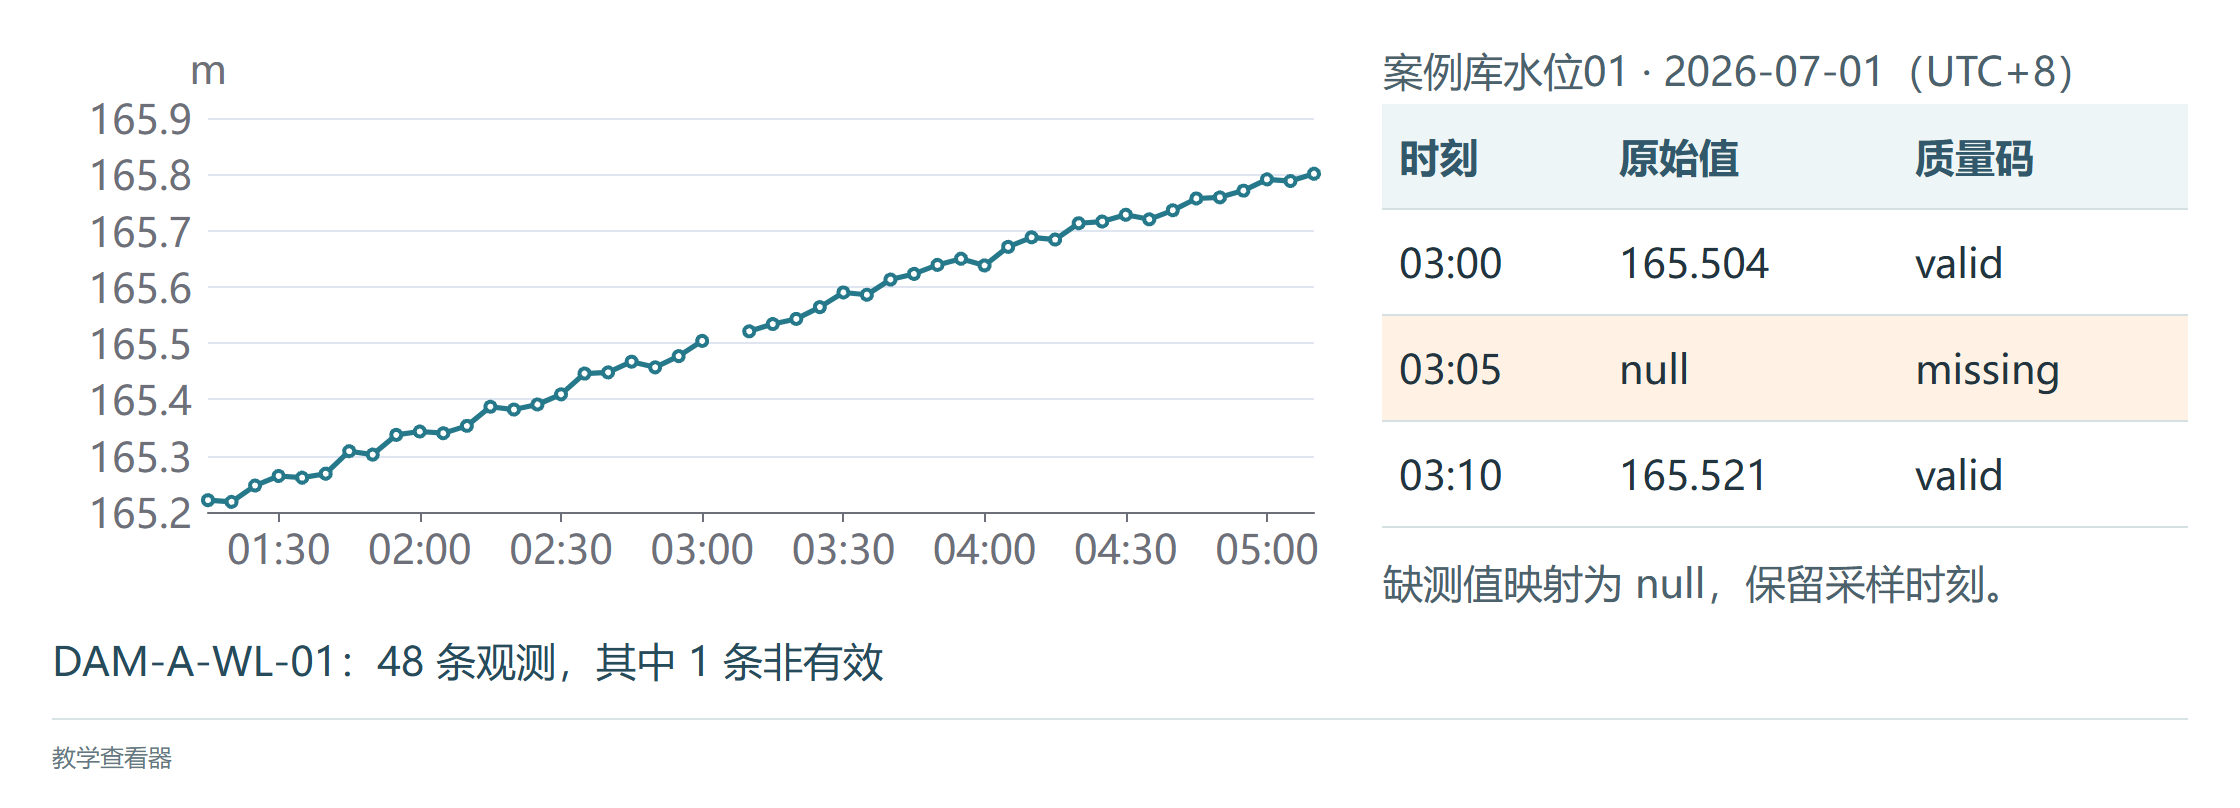
\includegraphics[width=16cm]{images/runtime/s5-missing-gap.png}
\caption{缺测记录与曲线断线逐项核对（教学查看器，调用S5曲线模块）}
\label{fig:ch07-gap-results}
\end{figure}

\paragraph{故障练习}把\texttt{toChartPoints}里的\texttt{null}临时改成\texttt{0}，刷新后再选 WL-01。纵轴被迫从0画起，03:05处出现一根直插到底的尖刺，其余时段一米多的涨幅被压成一条几乎水平的线。一个缺测点就足以毁掉整张图的可读性。改回\texttt{null}，再试另一种错误：在\texttt{map}之前加上\texttt{.filter(item => item.quality !== 'missing')}，曲线变成连续的一条，03:00与03:10被直接连上，缺测从图上消失了。两种写法都不会报错，只能靠对照原始记录发现。

\paragraph{给可疑点换个形状}选中 WL-02（把上面命令里的编码改成\texttt{DAM-A-WL-02}），17:35处有一个173.2\,m的尖峰，状态文字提示有1条非有效观测，但图上这个点与其他点长得一样。\texttt{toChartPoints}已经把质量码放在每个数据点上，只需在系列配置里加两项：

\begin{lstlisting}[label={lst:ch07-suspect-symbol},language=JavaScript,breaklines=true,caption={可疑点改用菱形并放大（加在 series 配置中）}]
symbol: (value, params) =>
  params.data.quality === 'suspect' ? 'diamond' : 'circle',
symbolSize: (value, params) =>
  params.data.quality === 'suspect' ? 12 : 4,
\end{lstlisting}

清单\ref{lst:ch07-suspect-symbol}加在\texttt{series-controller.js}中\texttt{setOption}的系列配置里，与\texttt{showSymbol}并列。刷新后17:35的点变成一个较大的菱形，数值和位置不变。这里用形状而不用红色，是因为红色已经留给了预警等级。可疑点没有被删除：这个173.2\,m会把纵轴撑高，这正是值班员需要看到的现象。

\paragraph{给缺测段加阴影}只有一个点缺测时，断口很窄，容易看漏。清单\ref{lst:ch07-missing-disconnect}在生成数据点的同时找出连续的缺测区间，用\texttt{markArea}画成灰色阴影，对应图\ref{fig:ch07-missing-gap}中的灰色块。\texttt{gridTimes}是按采样周期生成的完整时间轴，\texttt{readingByTime}是按时间索引的观测；在时间轴上找不到记录的时刻同样按缺测处理，这样后端漏发记录时也能看到缺口。

\begin{lstlisting}[label={lst:ch07-missing-disconnect},language=JavaScript,breaklines=true,caption={质量码驱动的缺测断线与阴影区间}]
function toSeriesPoint(reading, time) {
  const value = reading?.value;
  const quality = reading?.quality ?? 'missing';
  return quality === 'missing' ? [time, null] : [time, value];
}

function buildSeries(times, byTime) {
  const data = times.map(t => toSeriesPoint(byTime.get(t), t));
  const gaps = [];
  let start = null;
  for (let i = 0; i < times.length; i += 1) {
    if (data[i][1] === null && start === null) start = times[i];
    if (data[i][1] !== null && start !== null) {
      gaps.push([{xAxis: start}, {xAxis: times[i - 1]}]);
      start = null;
    }
  }
  if (start !== null) gaps.push([{xAxis: start}, {xAxis: times.at(-1)}]);
  return {data, gaps};
}

const {data, gaps} = buildSeries(gridTimes, readingByTime);
chart.setOption({series: [{id: 'level', data, connectNulls: false,
  markArea: {itemStyle: {color: 'rgba(120,120,120,.12)'}, data: gaps}}]});
\end{lstlisting}

\paragraph{自测}水位曲线的纵轴为什么通常不从0开始？渗压曲线呢？答案要点：库水位是相对高程基准的高程值，0\,m没有物理意义，变化幅度相对绝对值很小，从0起画看不出变化。渗压同理。雨量柱状图则必须从0开始，因为柱的长度就是雨量。

\subsection{追加新观测与切换序列}

曲线画出来以后，新观测还会不断到达。最直接的做法是每来一条就重新调用一次\texttt{setOption}。ECharts 默认会把新配置与旧配置合并：\texttt{series}按\texttt{id}匹配，只更新你提供的字段，坐标轴、标题等没提到的部分保持原样。所以追加一条观测时，只需要提交带\texttt{id}的新数据数组。合并也有副作用：想删掉一条已经不存在的序列，只提交剩下的序列是删不掉的，旧序列会继续留在图例和提示框里，这时要用\texttt{replaceMerge:['series']}明确要求替换整个序列集合。表\ref{tab:ch07-echarts-update}对照三种更新方式。

\begin{table}[htbp]
\centering
\caption{ECharts三种更新方式与适用边界}
\label{tab:ch07-echarts-update}
\begin{tabular}{p{3.0cm}p{4.2cm}p{5.0cm}}
\toprule
方式 & 关键调用 & 适用场景与注意事项 \\
\midrule
局部合并 & \texttt{setOption(option)} & 默认按\texttt{id}合并；保留未提供的配置，适合更新已有序列数据 \\
替换集合 & \texttt{replaceMerge} & 删除或重排序列时使用；必须重新提供完整序列集合 \\
流式追加 & \texttt{appendData(...)} & 限支持的系列且不用\texttt{dataset}；水位折线用局部合并，排序、去重和窗口裁剪由应用层处理 \\
\bottomrule
\end{tabular}
\end{table}

表中的\texttt{appendData}是 ECharts 的增量渲染接口，只有部分系列支持，例如\texttt{scatter}和\texttt{lines}，并且不能与\texttt{dataset}一起用；\texttt{lines}是线段系列，与本章画过程线用的\texttt{line}不是一回事\cite{apacheECharts}。水位折线的更新走局部合并。

清单\ref{lst:ch07-append-data}是配套工程的\texttt{frontend/src/lesson74/window-chart.js}。调用方传入一个已经初始化的图表，得到两个函数：\texttt{appendTail}在收到一条新观测时调用，\texttt{replaceWithTwoSeries}在需要同时显示水位和雨量时调用。

\begin{lstlisting}[label={lst:ch07-append-data},language=JavaScript,breaklines=true,caption={水位折线的尾部更新与序列切换}]
export function createWindowChart(chart) {
  let points = [];
  function replaceWithTwoSeries(level, rain) {
    points = level.slice(-300);
    chart.setOption({
      legend: {data: ['库水位', '时段雨量']},
      xAxis: {type: 'time'},
      yAxis: [{type: 'value', name: '水位/m'},
              {type: 'value', name: '雨量/mm'}],
      series: [
        {id: 'level', name: '库水位', type: 'line',
         yAxisIndex: 0, connectNulls: false, data: points},
        {id: 'rain', name: '时段雨量', type: 'bar',
         yAxisIndex: 1, data: rain.slice(-300)}
      ]
    }, {replaceMerge: ['series'], lazyUpdate: true});
  }
  function appendTail(reading) {
    const value = reading.quality === 'missing' ? null : reading.value;
    points = [...points, [reading.occurredAt, value]].slice(-300);
    chart.setOption({series: [{id: 'level', data: points}]});
  }
  replaceWithTwoSeries([], []);
  return {appendTail, replaceWithTwoSeries};
}
// 页面调用：const live = createWindowChart(chart);
// 收到下一条观测时调用 live.appendTail(reading)。
\end{lstlisting}

这段代码有三处值得注意。第一，数据缓冲\texttt{points}放在模块自己的变量里，图表只负责显示。要加阈值线、要重新排序，改的都是这份缓冲，不必去读图表内部的状态。第二，\texttt{slice(-300)}让缓冲最多保留300个点，超出的旧点被丢弃。对5\,min采样的水位，300点约为25\,h；需求若是“固定显示最近24小时”，要按时间戳裁剪。第三，\texttt{appendTail}假定观测按时间递增到达。迟到的观测不能直接追加到尾部，要先在缓冲里按\texttt{occurredAt}排序、去掉重复的\texttt{eventId}，再整体提交。

\texttt{replaceWithTwoSeries}给水位和雨量各配一根纵轴，单位分别写在轴名里，并用\texttt{replaceMerge}替换序列集合。在\texttt{frontend/}执行\texttt{npx vitest run tests/window-chart.test.js}可以看到两个检查：追加超过300条后缓冲只剩末尾300点，其中的\texttt{missing}点仍是空值；切换为双序列后两根轴的单位不同，之后的追加不会破坏新窗口。

\subsection{图表选型与双轴图}

折线之外还有很多图形可选。选图的依据是读者要完成的任务：比较、看趋势、看分布，还是定位。表\ref{tab:ch7-task-chart}按任务列出优先选用的图形，并各举一个案例水库的例子。

\begin{table}[htbp]
\centering
\caption{业务任务与图型选择决策表}
\label{tab:ch7-task-chart}
\begin{tabular}{p{2.0cm}p{3.3cm}p{4.0cm}p{3.3cm}}
\toprule
任务 & 读者要回答的问题 & 优先图型与视觉变量 & 案例水库示例 \\
\midrule
比较 & 哪个测点更高或变化更大？ & 排序条形图、点图；位置、长度 & 12个渗压测点当前值排序 \\
趋势 & 数值如何随时间变化？ & 折线图、面积图；位置、线型 & PZ-07渗压与库水位过程 \\
分布 & 数据集中还是离散？ & 直方图、箱线图、蜂群图；位置、面积 & 位移测点日变化分布 \\
构成 & 总量由哪些部分组成？ & 堆叠条形图、面积图；长度、明度 & 分时段降雨量与累计量 \\
相关 & 两个量是否同步变化？ & 散点图、热力图；位置、大小 & 水位与渗压的相关关系 \\
定位 & 异常发生在哪里？ & 专题地图、符号图、三维标注；位置、形状 & 坝段测点和影响范围 \\
\bottomrule
\end{tabular}
\end{table}

表中“视觉变量”一栏来自 Bertin 对图形符号的分类：位置、长度、角度、面积、明度、色相、纹理、形状和方向。它们表达数量的准确程度不同。人眼比较位置和长度最准，角度其次，面积和明度要靠估计，色相适合区分类别，不适合表达大小。粗略记为“位置 $>$ 长度 $>$ 角度 $>$ 面积 $>$ 颜色”。把水位差异画在纵轴位置上，比用一组深浅相近的颜色更容易读准。一个视觉变量只承担一种含义：如果颜色既表示预警等级又表示数据质量，可疑数据看上去就像高风险数据。7.1.2节把质量交给形状和断线、把颜色留给预警等级，依据就在这里。

设计一张图可以按五个问题依次回答：读者要做什么判断；需要哪些字段、单位、时间窗和质量码；用哪种图形和视觉变量；提供哪些交互，它们改变的是视图还是查询条件；图例、数据版本和生成时间怎样让读者能复核。一个页面可以同时有趋势图和定位图，它们共享对象编码和过滤条件：用户在图表里选中 PZ-07，三维场景里显示的就是同一个测点、同一个时间窗。

\paragraph{雨量与水位的双轴图}分析降雨与库水位的关系时，常把雨量柱和水位线画在一张图上。图\ref{fig:ch7-rain-level-combo}是水文上惯用的画法：雨量柱从上方的零基线向下画，读左轴；水位线读右轴；两者共用横轴的观测时刻。雨量倒挂可以避免柱子遮挡水位线，向下的柱形表示的仍是非负的雨量。

\begin{figure}[htbp]
\centering
\begin{tikzpicture}[x=1cm,y=1cm,>=Stealth,font=\scriptsize]
\foreach \y in {0,1,2,3,4}{\draw[TextGray!15] (0,\y)--(10,\y);}
\draw[->,TextGray] (0,4.2)--(0,-.18);
\draw[->,TextGray] (10,-.05)--(10,4.2);
\draw[TextGray] (0,0)--(10,0);
\node[text=TextGray] at (10.65,-.4) {时刻};
\node[text=Accent!80!black,above] at (0,4.35) {雨量/mm（向下增大）};
\node[text=PrimaryDark,above] at (10,4.35) {水位/m（向上增大）};
\foreach \y/\v in {4/0,3/5,2/10,1/15,0/20}{\draw[TextGray] (0,\y)--(-.1,\y) node[left]{\v};}
\foreach \y/\v in {0/163.5,1/164.0,2/164.5,3/165.0,4/165.5}{\draw[TextGray] (10,\y)--(10.1,\y) node[right]{\v};}
\foreach \x/\v in {1/0,3/8.4,5/16.2,7/4.8,9/0}{
  \filldraw[fill=Accent!28,draw=Accent] (\x-.25,4) rectangle (\x+.25,4-.2*\v);
}
\draw[Primary,line width=1.2pt] (1,1.4)--(3,1.6)--(5,2.4)--(7,3.2)--(9,3.0);
\foreach \x/\y in {1/1.4,3/1.6,5/2.4,7/3.2,9/3.0}{\filldraw[fill=white,draw=Primary] (\x,\y) circle(2pt);}
\foreach \x/\t in {1/08:00,3/10:00,5/12:00,7/14:00,9/16:00}{\draw[TextGray] (\x,0)--(\x,-.1) node[below]{\t};}
\node[text=TextGray,align=center] at (5,-.85) {橙柱：时段雨量，零基线在上方；蓝线：库水位，读取右轴\\数据与本节ECharts清单一致，两个纵轴共用观测时刻};
\end{tikzpicture}
\caption{雨量倒挂柱与水位过程线的双轴组合示意}
\label{fig:ch7-rain-level-combo}
\end{figure}

清单\ref{lst:ch07-rain-level-dualaxis}给出与图\ref{fig:ch7-rain-level-combo}数据一致的配置，在任何一个已初始化的图表上调用即可。与7.2.2节\texttt{replaceWithTwoSeries}的双轴相比，变化在于雨量轴的\texttt{inverse:true}和轴标签上的单位；水位轴设了\texttt{min}，是因为五个水位值都在164\,m以上。

\begin{lstlisting}[label={lst:ch07-rain-level-dualaxis},language=JavaScript,breaklines=true,caption={雨量倒挂柱与水位过程线的配置}]
const times = ['08:00', '10:00', '12:00', '14:00', '16:00'];
const rain = [0, 8.4, 16.2, 4.8, 0];
const level = [164.2, 164.3, 164.7, 165.1, 165.0];

chart.setOption({
  legend: {data: ['时段雨量', '库水位']},
  tooltip: {trigger: 'axis'},
  xAxis: {type: 'category', data: times, name: '观测时刻'},
  yAxis: [
    {type: 'value', name: '雨量/mm', inverse: true,
      min: 0, axisLabel: {formatter: '{value} mm'}},
    {type: 'value', name: '水位/m', min: 163.5,
      axisLabel: {formatter: '{value} m'}}
  ],
  series: [
    {name: '时段雨量', type: 'bar', yAxisIndex: 0,
      data: rain, barMaxWidth: 28},
    {name: '库水位', type: 'line', yAxisIndex: 1,
      data: level, showSymbol: true, smooth: false}
  ]
}, true);
\end{lstlisting}

双轴图容易造成误读，三个反例值得动手试一遍。第一，把水位轴的最小值从163.5\,m改成164\,m，曲线看起来波动大了很多，实际变化量没有变，所以轴范围要写在图上。第二，雨量按小时聚合而水位按5\,min采样时，两者的峰值会错位；要么在服务端统一时间桶，要么在图例里分别标出采样周期。第三，两条曲线在图上“同步”可能只是两根轴的比例凑巧，图形本身不说明因果关系。若目的是比较不同测点的绝对值，改用上下排列的分面图或同一根轴，比双轴更稳妥。

\subsection{图表与三维对象的双向联动}

联动要解决的问题是：图表库只认识数据点的下标，三维引擎只认识网格对象，两边都不知道“测点”是什么。把两者连起来的是\texttt{assetId}。第6章绑定测点时把它写进了每个小球的\texttt{userData.assetId}，观测记录里也带着同名字段。图\ref{fig:chart-technology-selection}画出三者的分工：ECharts 负责二维曲线，Three.js 负责三维场景，两者之间不直接调用，选中了哪个对象、关注哪个时刻，都经过一个联动控制器转发。联动逻辑如果写进图表一侧或场景一侧，两个库就互相依赖了，日后替换其中之一时要同时改动两边。

\begin{figure}[htbp]
\centering
\begin{tikzpicture}[node distance=8mm and 14mm,
  tech/.style={draw=Primary,rounded corners,fill=PrimaryLight,align=center,
    minimum width=2.6cm,minimum height=.9cm}]
\node[tech] (data) {统一展示记录};
\node[tech,below left=of data] (chart) {Apache ECharts\\趋势与统计};
\node[tech,below right=of data] (three) {Three.js\\空间与状态};
\node[tech,below=18mm of data] (link) {联动控制器\\对象ID+时间窗};
\draw[->,draw=Primary,thick] (data)--(chart);
\draw[->,draw=Primary,thick] (data)--(three);
\draw[<->,draw=Accent,thick] (chart)--(link);
\draw[<->,draw=Accent,thick] (three)--(link);
\end{tikzpicture}
\caption{图表、三维场景与联动控制器的职责}
\label{fig:chart-technology-selection}
\end{figure}

两个方向各用到一个库接口。从图表到场景：ECharts 的点击事件参数\texttt{params}里，\texttt{params.data}是被点中的数据点，\texttt{params.dataIndex}是它在序列中的下标，控制器据此找到观测记录，取出\texttt{assetId}和\texttt{occurredAt}，调用场景的高亮接口。从场景到图表：拾取到的三维对象带着\texttt{userData.assetId}，控制器查到它对应的数据下标，用\texttt{dispatchAction}让图表高亮该点并显示提示框。清单\ref{lst:ch07-link-controller}是配套工程的\texttt{frontend/src/lesson74/link.js}。

\begin{lstlisting}[label={lst:ch07-link-controller},language=JavaScript,breaklines=true,caption={ECharts与Three.js对象的双向联动控制器}]
function createLinkController(chart, scene, readings) {
  const byAsset = new Map(readings.map((r, i) => [r.assetId, {i, r}]));
  const onChartClick = params => {
    const point = params.data?.assetId
      ? params.data : readings[params.dataIndex];
    if (!point) return;
    scene.focusAsset(point.assetId, point.occurredAt);
  };
  const onSceneSelect = object => {
    const assetId = object.userData.assetId;
    const hit = byAsset.get(assetId);
    if (!hit) return;
    chart.dispatchAction({type: 'highlight', seriesId: 'level', dataIndex: hit.i});
    chart.dispatchAction({type: 'showTip', seriesId: 'level', dataIndex: hit.i});
  };
  chart.on('click', onChartClick);
  // scene 是应用层的场景封装对象（带事件总线），
  // 不是 THREE.Scene 本身——后者没有 on/off 接口
  scene.on('select', onSceneSelect);
  return () => {
    chart.off('click', onChartClick);
    scene.off('select', onSceneSelect);
  };
}
\end{lstlisting}

读这段代码时注意四点。
\begin{itemize}
\item \texttt{onChartClick}先看数据点自己有没有\texttt{assetId}，没有就用下标到\texttt{readings}里取。阶段页的数据点由\texttt{toChartPoints}生成，不带\texttt{assetId}，走的是后一条路；下标越界时\texttt{point}为空，函数直接返回。
\item \texttt{byAsset}按\texttt{assetId}建索引。阶段页一次只显示一个测点的观测，所有记录的\texttt{assetId}相同，\texttt{Map}里留下的是最后一条，所以点球以后图表高亮的是该测点最新的一次观测。
\item \texttt{scene}参数不是\texttt{THREE.Scene}。Three.js 的场景对象没有\texttt{on}、\texttt{off}这样的事件接口，这里传入的是应用层的一个封装，由\texttt{src/lesson74/scene-bus.js}提供：它维护事件订阅，实现\texttt{focusAsset}（把指定测点的球改成橙色、把上一个改回蓝色），并在用户点中三维对象时广播\texttt{select}事件。
\item 函数返回一个解绑函数。切换测点或离开页面时必须调用它，否则每切换一次就多一组点击处理器，点一下曲线会触发多次高亮。
\end{itemize}

\paragraph{S5 阶段页的装配}\texttt{lesson74.html}的入口\texttt{src/lesson74/main.js}把几个模块装在一起：复用 S4 的场景和测点绑定，创建\texttt{sceneBus}，用7.4.1节的拾取器把画布点击变成\texttt{select}事件，再由\texttt{series-controller.js}在每次选中时取数、画曲线、建立联动。数据来自教学接口，也可以换成 S3 的完整后端。运行后点一个蓝色小球，右侧曲线切到该测点，球变橙色；点曲线上任意一个数据点，对应的球保持高亮；点坝体或空白处，状态文字提示“未选中测点”。图\ref{fig:ch07-scene-chart}是点中 PZ-07 后的画面，右侧是它在2026年7月1日的288条渗压观测。核对联动是否正确，看三样东西：对象编码、时间范围和单位（kPa）是否都属于被点中的测点。

\begin{figure}[htbp]
\centering
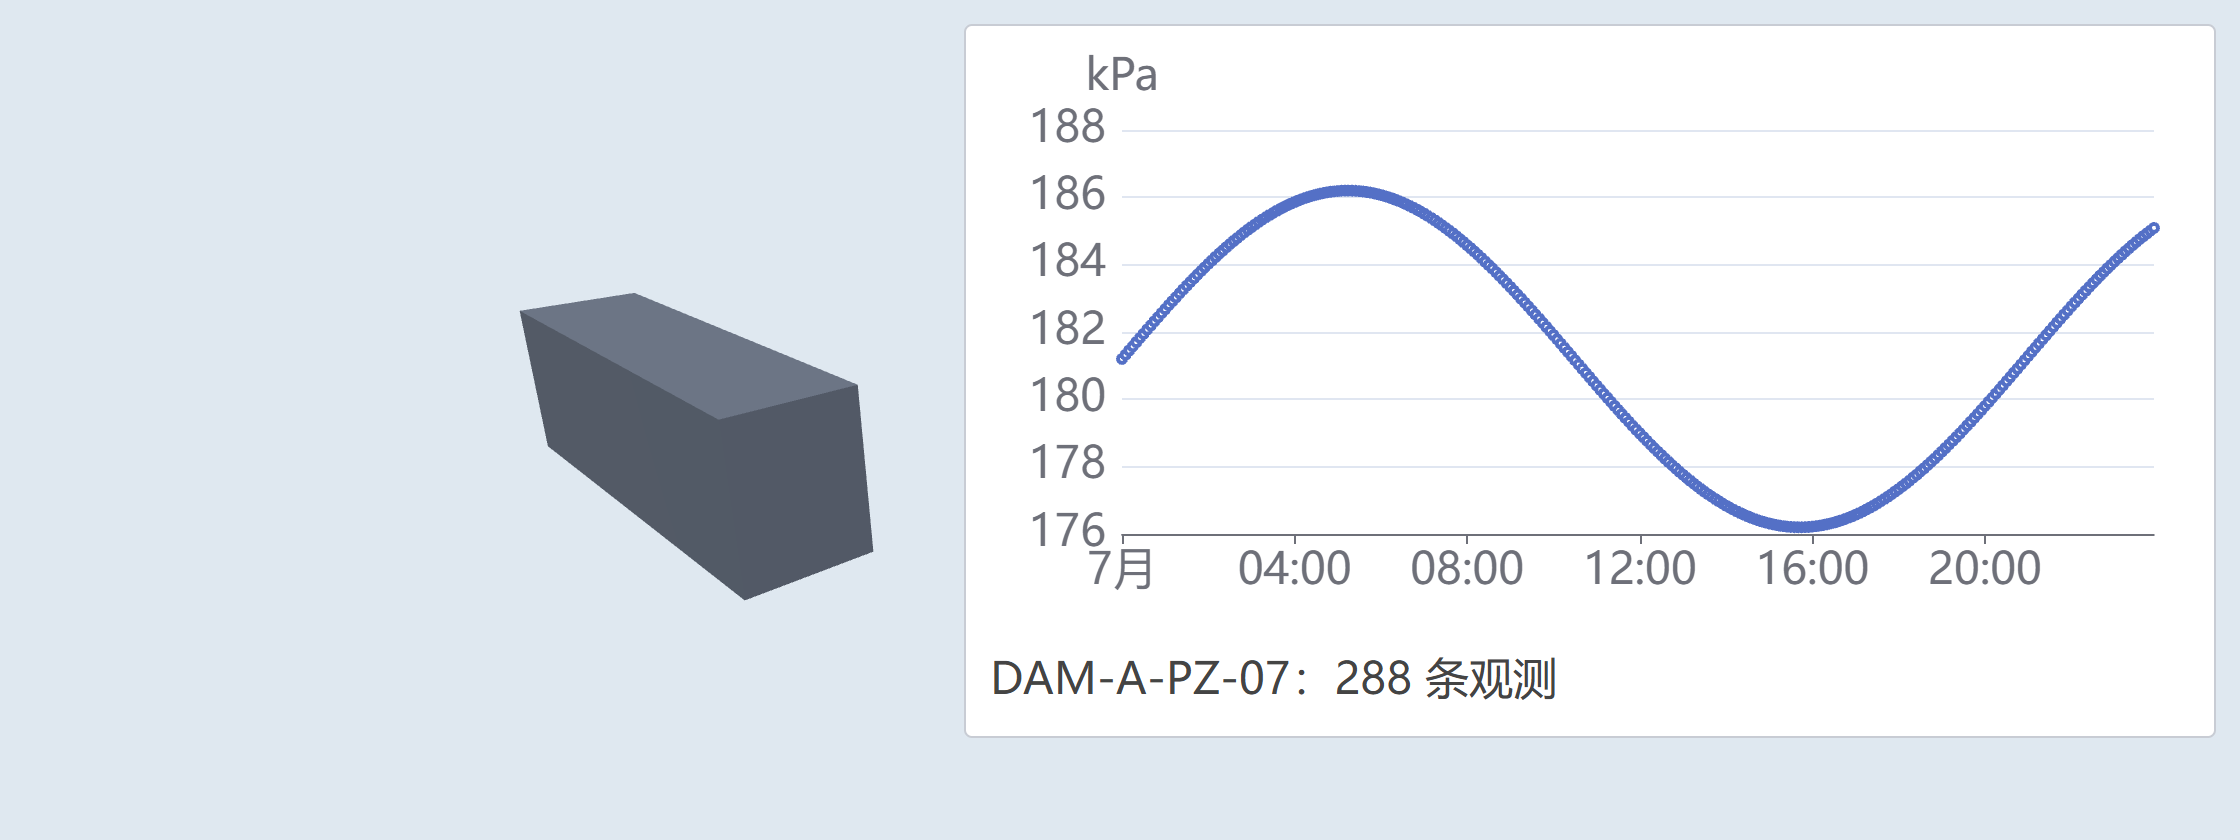
\includegraphics[width=16cm]{images/runtime/s5-scene-chart.png}
\caption{三维测点与渗压曲线联动（配套程序运行图，添加坐标识读标记）}
\label{fig:ch07-scene-chart}
\end{figure}

\paragraph{快速切换时的竞态}用户连点两个测点时，先发出的请求可能后返回。\texttt{series-controller.js}复用4.5.4节的做法：每次切换先让序号加1、取消上一个请求、解除旧联动并清空曲线，请求返回后核对序号，只有序号仍是最新的结果才允许更新曲线、单位和状态文字，并建立新的联动。解绑放在切换一开始，而不是放在请求成功之后，这样即使新请求失败或返回空结果，旧曲线也已经无法响应点击。

\paragraph{故障验证与自测}在浏览器开发者工具里把网络调成慢速，先点一个渗压测点，立即再点一个库水位测点，最终的曲线、单位和状态文字应全部属于后点的那个。接着选一个位移测点（教学数据里位移没有观测），应显示“暂无观测”，此时点击图表区域不会有任何高亮。断开网络再选测点，应显示失败原因；恢复网络后重新选择可以重试。如果旧曲线又冒出来，或旧的点击处理器还在响应，检查序号核对和解绑是否写在了所有返回分支之前。\texttt{tests/series-controller.test.js}覆盖这些异常路径及页面卸载后才到达的响应，\texttt{tests/lesson74.test.js}验证对象映射、下标越界和拾取。自测：请求已经取消了，为什么还要核对序号？答案要点：取消只能中止尚未完成的网络请求，已经拿到应答、正在执行的后续代码撤不回来；只有当前选择对应的结果才有权更新界面。

\paragraph{多张图共用时间轴}水位、雨量和渗压分成上下几张图时，希望拖动其中一张的时间轴，另外几张跟着动。清单\ref{lst:ch07-connect-charts}给两个图表实例设置相同的\texttt{group}，再调用\texttt{echarts.connect}，缩放和提示框就会同步。

\begin{lstlisting}[label={lst:ch07-connect-charts},language=JavaScript,breaklines=true,caption={多图表缩放联动与组标识}]
const levelChart = echarts.init(document.querySelector('#level'));
const rainChart = echarts.init(document.querySelector('#rain'));
levelChart.group = 'case-reservoir-time';
rainChart.group = 'case-reservoir-time';
echarts.connect('case-reservoir-time');

function focusTime(chart, occurredAt) {
  chart.dispatchAction({type: 'dataZoom',
    startValue: occurredAt, endValue: Date.parse(occurredAt) + 6 * 3600 * 1000});
}
\end{lstlisting}

\texttt{connect}只同步视图范围。它不知道\texttt{assetId}，对象定位仍由联动控制器完成；它也不会替你对齐采样周期，雨量和水位共用时间轴以后，图例里仍要各自标明采样周期和聚合方法。

\subsection{响应式与异常状态}

\paragraph{尺寸变化与销毁}图表实例要占用画布、事件监听器和内存，用完要还。清单\ref{lst:ch07-responsive-dispose}在7.2.1节初始化的基础上补上尺寸监听与销毁，把这两件事收进一个\texttt{mountChart}函数；\texttt{subscribe}是调用方传入的数据订阅函数，接收一个“新观测到达时怎么办”的回调并返回退订函数，7.2.2节的\texttt{appendTail}可以直接作为这个回调。容器尺寸变化用\texttt{ResizeObserver}监听。只监听\texttt{window}的\texttt{resize}事件是不够的：侧栏收起时窗口大小没变，图表容器却变宽了。函数返回的清理函数依次解除数据订阅、停止尺寸监听、移除点击处理器、销毁实例，在 Vue 3 组件里由\texttt{onUnmounted}调用。漏掉销毁不会立刻出错，切换测点几百次之后页面才开始变卡，这类问题从单次截图里发现不了。

\begin{lstlisting}[label={lst:ch07-responsive-dispose},language=JavaScript,breaklines=true,caption={响应式尺寸与ECharts实例销毁}]
// subscribe(onReading) 由调用方提供：注册新观测到达时的回调，返回退订函数；
// onReading(reading) 可以直接用 7.2.2 节的 appendTail
function mountChart(container, option, subscribe, onReading) {
  const chart = echarts.init(container, null, {renderer: 'canvas'});
  const observer = new ResizeObserver(() => chart.resize());
  observer.observe(container);
  chart.setOption(option);
  const unsubscribe = subscribe(onReading);
  return () => {
    unsubscribe();
    observer.disconnect();
    chart.off('click');
    chart.dispose();
  };
}
\end{lstlisting}

图\ref{fig:ch07-echarts-lifecycle}把这个过程画成状态图：数据变化触发配置合并，容器变化只触发尺寸重算，组件卸载时先解除外部订阅再销毁图表。

\begin{figure}[htbp]
\centering
\begin{tikzpicture}[>=Stealth,font=\small,
  life/.style={draw=Primary,rounded corners,fill=PrimaryLight,align=center,
    minimum width=2.7cm,minimum height=.95cm,text=PrimaryDark}]
\node[life] (create) at (0,0) {创建实例\\初始化option};
\node[life] (active) at (3.8,0) {组件存续期间\\按事件响应};
\node[life] (update) at (8.5,1.55) {更新数据\\setOption/appendData};
\node[life] (resize) at (8.5,0) {调整尺寸\\chart.resize};
\node[life,fill=Accent!10,draw=Accent] (dispose) at (8.5,-1.55) {解除订阅与释放实例\\unsubscribe + dispose};
\draw[->,Primary,thick] (create)--(active);
\draw[->,Primary,thick] (active.north east)--node[above,sloped,font=\scriptsize]{数据变化} (update.west);
\draw[->,Primary,thick] (active)--node[above,font=\scriptsize]{容器变化} (resize);
\draw[->,Accent,thick] (active.south east)--node[below,sloped,font=\scriptsize]{组件卸载} (dispose.west);
\end{tikzpicture}
\caption{ECharts实例的创建、更新、响应式与销毁生命周期}
\label{fig:ch07-echarts-lifecycle}
\end{figure}

\paragraph{五种不同的“没有曲线”}图表区域一片空白时，用户需要知道原因。加载中、对象没有观测、时间窗内无数据、权限不足、接口失败，是五种不同的状态，各自对应不同的下一步动作：等待、换一个测点、调整时间范围、申请权限、重试。阶段页用状态文字区分了其中三种（“正在读取”“暂无观测”“读取失败”）。数据质量可疑不属于“没有曲线”，它在曲线上用点形表达，在状态文字里给出条数。

\paragraph{不同屏幕}值班室大屏同时呈现工程总览、关键曲线和预警列表，首屏先放需要处置的事项和数据新鲜度，技术指标放到展开之后。桌面端以查询和研判为主。移动端保留待办、定位和确认，复杂的多图比较留给桌面端。屏幕变小时调整的是信息的优先级，不是把所有组件等比缩小。

\subsection{时间窗口与LTTB降采样}

前面的曲线一天288个点，直接画没有问题。查看一年的5\,min水位时，点数超过十万，而图表的宽度只有一千多个像素，一列像素里挤着上百个点，多数点画了也看不见。这一小节讲两件事：时间窗口怎样控制取多少数据，点数仍然太多时怎样在不丢掉峰值的前提下减点。

\paragraph{时间窗口}实时曲线用滑动窗口，只保留最近一段时间，7.2.2节的300点缓冲就是一种。历史查询由后端按时间跨度和屏幕宽度选择聚合粒度：表\ref{tab:api-contract}的观测查询接口有可选参数\texttt{agg}，浏览器拿到的应该是已经聚合好的序列，而不是把多年原始数据下载到前端再压缩。窗口可以按点数定，也可以按时长定，两者含义不同（7.1.4节），图的标题里要写明是“300点（约25小时）”还是“最近24小时”。

\paragraph{为什么不能等间隔抽点}最省事的减点办法是每隔$k$个点取一个。它的问题是取哪个点只看位置不看数值：洪峰恰好落在两个被取点之间，就从图上消失了。按桶取平均值也不行，平均会把尖峰削平，而且画出来的数值不是任何一次真实观测。监测曲线最需要保留的恰恰是峰值、谷值和突变。

\paragraph{LTTB的做法}Largest-Triangle-Three-Buckets（LTTB）算法\cite{steinarsson2013lttb}的思路是：在每一小段里，留下那个“最突出”的点。设原始序列有$N$个点，要减到$m$个点（$m\ge3$）。首点和尾点直接保留，中间的$N-2$个点按顺序均分为$m-2$个桶，每个桶留一个点。处理第$k$个桶时，上一个桶已经选定的点记为$P_{\mathrm{prev}}$，下一个桶里所有点的横、纵坐标平均值构成一个虚拟点$\overline{P}_{C}$（最后一个桶没有下一桶，用尾点代替）。对当前桶里的每个候选点$P_{\mathrm{cand}}$，计算它与$P_{\mathrm{prev}}$、$\overline{P}_{C}$围成的三角形面积，留下面积最大的那个，它成为下一轮的$P_{\mathrm{prev}}$。

面积用两个向量的叉积计算。从$P_{\mathrm{prev}}$分别指向$P_{\mathrm{cand}}$和$\overline{P}_{C}$的向量为
$\boldsymbol a=(x_{\mathrm{cand}}-x_{\mathrm{prev}},\,y_{\mathrm{cand}}-y_{\mathrm{prev}})$和
$\boldsymbol b=(\bar{x}_{C}-x_{\mathrm{prev}},\,\bar{y}_{C}-y_{\mathrm{prev}})$，
三角形面积是它们张成的平行四边形面积的一半，$S=\frac12|a_xb_y-a_yb_x|$，展开并整理符号得

\[
  S=\frac{1}{2}\left|
 (x_{\mathrm{prev}}-\bar{x}_{C})(y_{\mathrm{cand}}-y_{\mathrm{prev}})
 -(x_{\mathrm{prev}}-x_{\mathrm{cand}})(\bar{y}_{C}-y_{\mathrm{prev}})
 \right|.
\]

$P_{\mathrm{prev}}$与$\overline{P}_{C}$的连线代表曲线在这一段的大致走向，面积大意味着候选点离这条连线远，也就是偏离走向最多的点。平缓段里各候选点面积都小，留哪个差别不大；有尖峰的桶里，峰顶的面积最大，会被留下。图\ref{fig:lttb-principle}画出一个桶的情形：两个候选点中，$P_{\mathrm{cand},2}$对应的橙色三角形面积更大，被选中。横轴是时间（毫秒）、纵轴是观测值，两者量纲不同，面积本身没有物理意义；但同一个桶内所有候选点共用一条底边，改变任一坐标轴的比例只是给所有面积乘上同一个系数，不影响谁最大。

\begin{figure}[htbp]
\centering
\begin{tikzpicture}[x=.95cm,y=.82cm,>=Stealth,font=\small]
\fill[Accent!9] (3.1,0) rectangle (6.3,4.05);
\fill[PrimaryLight!65] (6.3,0) rectangle (10.3,4.05);
\foreach \x in {3.1,6.3,10.3}{\draw[TextGray!45,dashed] (\x,0)--(\x,4.05);}
\node[text=Accent!80!black,font=\scriptsize] at (4.7,4.8) {当前桶：比较候选面积};
\node[text=PrimaryDark,font=\scriptsize] at (8.3,4.8) {下一桶：求平均点};
\draw[->,TextGray] (0,0)--(11,0) node[right]{时间};
\draw[->,TextGray] (0,0)--(0,4.3) node[above]{观测值};
\coordinate (prev) at (2.8,2.7);
\coordinate (cand) at (4.4,2.0);
\coordinate (chosen) at (5.2,3.7);
\coordinate (nextmean) at (8.4,2.58);
\fill[Accent!22] (prev)--(chosen)--(nextmean)--cycle;
\draw[TextGray!65] plot coordinates {(0.5,1.0)(1.2,1.4)(2,1.2)(2.8,2.7)(3.6,1.7)(4.4,2.0)(5.2,3.7)(6,2.2)(6.8,2.5)(7.6,1.4)(8.4,3.0)(9.2,2.6)(10,3.4)};
\foreach \x/\y in {.5/1,1.2/1.4,2/1.2,2.8/2.7,3.6/1.7,4.4/2,5.2/3.7,6/2.2,6.8/2.5,7.6/1.4,8.4/3,9.2/2.6,10/3.4}{\fill[TextGray] (\x,\y) circle(1.3pt);}
\draw[Primary,dashed] (prev)--(cand)--(nextmean)--cycle;
\draw[Accent,thick] (prev)--(chosen)--(nextmean)--cycle;
\fill[Primary] (prev) circle(2.4pt) node[above left]{$P_{\mathrm{prev}}$};
\fill[Primary] (cand) circle(2.4pt) node[below]{$P_{\mathrm{cand},1}$};
\fill[Accent] (chosen) circle(2.6pt) node[above]{$P_{\mathrm{cand},2}$};
\fill[PrimaryDark] ($(nextmean)+(-.06,-.06)$) rectangle ($(nextmean)+(.06,.06)$);
\node[text=PrimaryDark,anchor=north west] at ($(nextmean)+(.08,-.05)$) {$\overline{P}_{C}$};
\node[text=TextGray,font=\scriptsize,align=center] at (5.5,-.65) {灰线与小圆点：原始观测；橙色三角形：本桶最大面积候选\\下一桶平均点由桶内五个观测的时间与数值分别求均值得到};
\end{tikzpicture}
\caption{LTTB降采样的几何直觉}
\label{fig:lttb-principle}
\end{figure}

清单\ref{lst:ch07-lttb}是这个过程的数组实现，输入是\texttt{[x, y]}数组，\texttt{threshold}即$m$。外层循环每轮处理一个桶：先求下一桶的平均点\texttt{avg}，再在当前桶的下标范围内逐个算面积，记下最大者。

\begin{lstlisting}[label={lst:ch07-lttb},language=JavaScript,breaklines=true,caption={LTTB分桶与最大三角形选择}]
function lttb(points, threshold) {
  if (threshold >= points.length || threshold === 0) return points;
  const sampled = [points[0]];
  const every = (points.length - 2) / (threshold - 2);
  let a = 0;
  for (let i = 0; i < threshold - 2; i += 1) {
    const avgStart = Math.floor((i + 1) * every) + 1;
    const avgEnd = Math.min(Math.floor((i + 2) * every) + 1, points.length);
    const next = points.slice(avgStart, avgEnd);
    const avg = next.length ? next.reduce((s, p) => [s[0] + p[0], s[1] + p[1]], [0, 0])
      .map(v => v / next.length) : points[points.length - 1];
    const rangeStart = Math.floor(i * every) + 1;
    const rangeEnd = Math.floor((i + 1) * every) + 1;
    let best = rangeStart; let maxArea = -1;
    for (let j = rangeStart; j < rangeEnd; j += 1) {
      const area = Math.abs((points[a][0] - avg[0]) * (points[j][1] - points[a][1])
        - (points[a][0] - points[j][0]) * (avg[1] - points[a][1])) / 2;
      if (area > maxArea) { maxArea = area; best = j; }
    }
    sampled.push(points[best]); a = best;
  }
  sampled.push(points.at(-1)); return sampled;
}
\end{lstlisting}

\paragraph{为什么适合监测曲线，什么时候不能用}LTTB 有两个性质对监测数据有用。它留下的每个点都是一次真实观测，时间和数值都没有被改动，鼠标悬停时读到的是实测值。它优先保留峰、谷和转折，曲线的形态与原始曲线接近，值班员据此判断“有没有异常过程”不会被误导。

它的适用范围限于给人看的曲线。下面几种情况要回到原始观测。
\begin{itemize}
\item 预警判定和超限统计。一个超过阈值的点如果与一个更突出的点落在同一个桶里，就会被舍弃，用降采样后的序列做判定会漏报。最大值、平均值、超阈次数等统计同理，都从原始数据计算。
\item 审计取证和报表。降采样的结果与目标点数$m$有关，换一个屏幕宽度，留下的点就不同，不能作为可复现的依据。
\item 含缺测的序列。清单\ref{lst:ch07-lttb}假定每个点都有数值，\texttt{null}参与运算会被当作0。做法是先在缺测处把序列切成几段，各段分别降采样，段与段之间保留空值，断线因此不会丢失。
\item 雨量等时段累计量。柱的高度是时段总量，减点的正确做法是按更长的时段求和（7.1.4节），而不是挑几根柱子留下。
\end{itemize}
用户放大到某一小段时，可见点数减少，应当重新请求该时间段的原始或更细粒度的数据，而不是把降采样后的稀疏点放大了看。

\paragraph{ECharts内置的降采样}ECharts 的折线系列可以直接声明\texttt{sampling:'lttb'}，库在点数超过像素宽度时自动按上述方法减点，不必自己调用清单\ref{lst:ch07-lttb}。手写一遍的意义在于知道它做了什么、丢了什么。清单\ref{lst:ch07-window-options}是历史曲线的系列配置，在7.2.1节的配置基础上增加了四样东西：\texttt{sampling}声明降采样；\texttt{dataZoom}提供滚轮缩放和底部滑块，改变可见时间范围；\texttt{markLine}在168.0\,m处画出正常蓄水位，\texttt{markArea}标出165.0\,m至168.0\,m的区间；\texttt{visualMap.pieces}按数值区间给曲线分段着色。\texttt{progressive}一组参数让点数很多的序列分批绘制。

\begin{lstlisting}[label={lst:ch07-window-options},language=JavaScript,breaklines=true,caption={历史曲线的降采样、缩放与阈值带}]
const historyOption = {
  animation: false,
  dataZoom: [
    {type: 'inside', xAxisIndex: 0, filterMode: 'none'},
    {type: 'slider', xAxisIndex: 0, height: 18}
  ],
  visualMap: {show: false, dimension: 1, pieces: [
    {lte: 165.0, color: '#1976D2'},
    {gt: 165.0, lte: 168.0, color: '#F9A825'},
    {gt: 168.0, color: '#C62828'}
  ]},
  series: [{id: 'level', type: 'line', sampling: 'lttb',
    showSymbol: false, progressive: 5000, progressiveThreshold: 10000,
    data: historyPoints,
    markLine: {data: [{yAxis: 168.0, name: '正常蓄水位'}]},
    markArea: {data: [[{yAxis: 165.0}, {yAxis: 168.0}]]}}]
};
chart.setOption(historyOption);
\end{lstlisting}

图上的参考线和分段颜色只帮助读图。某个水位是否触发预警，由第8章的规则读取原始数值、质量码和当前工况来判定；图上的线要注明它是什么水位、来自哪个版本的参数，一条没有出处的红线容易被当成预警阈值。

\subsection{渲染器、性能预算与更新节奏}

\paragraph{Canvas还是SVG}\texttt{echarts.init}的第三个参数可以选渲染器。Canvas 把整张图画在一个位图上，节点数不随数据点增长，适合连续折线、数千个点和频繁刷新。SVG 为每个图形生成一个 DOM 节点，适合图形少、需要逐个获得键盘焦点或高质量打印的页面，节点过多时布局和事件开销会明显上升。本章的曲线都用 Canvas。

\paragraph{大数据量开关的代价}散点或柱形数量很大时，\texttt{large:true}和\texttt{largeThreshold}让 ECharts 批量绘制，代价是逐点样式和鼠标事件减少，需要点击单个测点的图不适合打开它，应先在服务端聚合或按缩放级别分层。\texttt{progressive}与\texttt{progressiveThreshold}把绘制拆成若干批，先保证页面能响应；分批期间坐标轴、阈值带和缺测阴影要先画出来，避免用户先看到一条没有质量提示的曲线。这些开关都不改变数据，也都不能代替服务端聚合。

\paragraph{更新节奏}5\,min采样的数据没有必要来一条重绘一次。同一测点在100--200\,ms内到达的多条补传可以合并后只提交一次\texttt{setOption}；同一时刻到达的多个测项，先按\texttt{assetId}分组、排序、去重，再一次提交。坐标轴、图例和事件监听器在初始化时声明一次，每条消息里只更新数据数组，不要反复创建格式化函数和样式对象。用户正在拖动时间轴时，后台到达的更新先放进缓冲，松手后再合并，避免更新与交互争用主线程。需要立即呈现的红色预警走单独的通知通道，不排在普通曲线更新后面。

判断“卡在哪里”要分段测量：消息到达到通过校验的时间、\texttt{setOption}的耗时、浏览器绘制的耗时。页面上同时记录最后一次有效观测时间、最后一次收到消息的时间和最后一次成功绘制的时间，就能区分是传感器没有数据、网络没有消息，还是浏览器没有画出来。缩放时的查询缓存、断线后的状态恢复和成套的回归数据，见附录C的\ref{app:ext-ch07-chart-runtime}节。

\subsection{专题地图的表达方式}

专题地图把数值、类别和空间关系叠加到同一张底图上，回答“哪里”的问题。常用的有四种图层。等值线表达连续场的等值边界，例如水位面、降雨量或淹没深度。色斑图把栅格或分区的数值映射为连续色带，适合观察空间梯度，要标明分级方法、单位和缺测区域。流向箭头用方向和长度表达水流或输水路径，箭头密度随屏幕尺度调整。站点符号用位置、形状和边框表达测点、闸门、雨量站或网关的状态，适合点击查询和联动。图\ref{fig:ch7-thematic-map}把四种图层画在一张图上；实际使用时每一层有独立的图例和开关，避免底图颜色与专题色带互相干扰。

\begin{figure}[htbp]
\centering
\begin{tikzpicture}[x=1cm,y=.8cm,>=Stealth,font=\scriptsize]
\fill[Primary!8] (0,0) rectangle (10,5);
\fill[Primary!18] (0,1.1) .. controls (2,1.8) and (3,1.0) .. (5,1.6)
  .. controls (7,2.2) and (8,1.2) .. (10,1.8)--(10,5)--(0,5)--cycle;
\fill[Primary!30] (0,2.7) .. controls (2,3.4) and (3,2.3) .. (5,2.9)
  .. controls (7,3.7) and (8,2.6) .. (10,3.2)--(10,5)--(0,5)--cycle;
\draw[Primary] (0,0) rectangle (10,5);
\draw[PrimaryDark!75,dashed] (0,1.1) .. controls (2,1.8) and (3,1.0) .. (5,1.6)
  .. controls (7,2.2) and (8,1.2) .. (10,1.8);
\draw[PrimaryDark!75,dashed] (0,2.7) .. controls (2,3.4) and (3,2.3) .. (5,2.9)
  .. controls (7,3.7) and (8,2.6) .. (10,3.2);
\foreach \a/\b/\c/\d in {1/4.5/2.8/3.9,3.3/3.65/5.1/3.05,5.6/2.8/7.4/2.2}{\draw[Accent!85!black,line width=1.1pt,->] (\a,\b)--(\c,\d);}
\foreach \x/\y/\s in {1.2/1.4/A,3.4/2.4/B,6.2/3.8/C,8.4/1.1/D}{
  \filldraw[fill=white,draw=PrimaryDark,thick] (\x,\y) circle(2.6pt);
  \node[above,text=PrimaryDark] at (\x,\y) {\s};
}
\node[text=Accent!85!black] at (5,4.65) {箭头：流向};
\foreach \x/\c in {0/8,.45/18,.9/30}{\fill[Primary!\c] (\x,-.6) rectangle (\x+.45,-.35);}
\node[anchor=west,text=TextGray] at (1.55,-.47) {连续场：由浅至深表示低到高（示意）};
\node[anchor=west,text=TextGray] at (0,-1.05) {虚线：等值线\qquad 带字母圆点：监测站点};
\end{tikzpicture}
\caption{等值线、色斑图、流向箭头与站点符号的组合表达}
\label{fig:ch7-thematic-map}
\end{figure}

色带的分级固定在服务端或配置文件里，图例显示最小值、最大值、单位和时间窗。用户缩放时可以改变符号大小和标签密度，数值分级保持不变，否则同一个颜色在两次缩放之间代表不同的数值。缺测区域用独立的纹理或灰色遮罩，不用低值的颜色代替“没有数据”。

清单\ref{lst:ch07-thematic-layer}用 ECharts 的\texttt{geo}组件画站点符号图。质量与预警仍然分开表达：可疑点改变形状，预警等级决定颜色，缺测点不进入数值散点。\texttt{warningLevelColor}由预警服务返回的等级经7.2.9节的色板换算而来，展示层自己不判定等级。

\begin{lstlisting}[label={lst:ch07-thematic-layer},language=JavaScript,breaklines=true,caption={专题地图图层与站点符号配置}]
const stationLayer = readings
  .filter((item) => item.quality !== 'missing')
  .map((item) => ({
    name: item.assetId,
    value: [item.lon, item.lat, item.value],
    symbol: item.quality === 'suspect' ? 'diamond' : 'circle',
    itemStyle: {color: item.warningLevelColor},
    label: {show: item.selected === true, formatter: item.assetId}
  }));

const thematicOption = {
  tooltip: {trigger: 'item'},
  // geo 组件是 coordinateSystem:'geo' 的前提：需先用
  // echarts.registerMap('case-reservoir', geoJson) 注册库区边界
  geo: {map: 'case-reservoir', roam: true,
    itemStyle: {areaColor: '#f4f6f8', borderColor: '#9aa5b1'}},
  visualMap: {min: 0, max: 100, dimension: 2,
    text: ['高', '低'], calculable: true},
  series: [{type: 'scatter', coordinateSystem: 'geo',
    data: stationLayer, symbolSize: 10}]
};
\end{lstlisting}

发布地图前核对两件事。位置是否正确：底图、专题图层和测点要使用同一坐标参考系；站点位置正确而色斑图整体偏移时，先查栅格范围、轴序和瓦片矩阵，不要在前端给点位加一个固定偏移。数值是否正确：抽样读取栅格或要素的属性，与生成地图时的时间窗、单位和版本对照。底图若来自只返回图片的 WMS 服务，专题数值仍要从可查询的要素服务或覆盖服务取得，不能从图片像素反推监测值。站点符号的点击事件回传\texttt{assetId}，显示用的标签不能当主键用。

\subsection{色彩体系与可读性}

\paragraph{三类色板}色板的类型取决于数据表示的是数量、偏差还是类别。顺序型色板用于从低到高的单调量，例如雨量、淹没深度，明度或饱和度沿一个方向变化。发散型色板用于有明确中心的偏差，例如渗压相对基线的升降，中心用中性色，两端用对比色。定性色板用于没有顺序的类别，例如渗压、位移、水位、雨量四类测项，颜色之间不暗示高低。混用的后果是读者把类别颜色读成数值大小，或者把接近中心的偏差看成“没有数据”。

彩虹色阶在水利看板里很常见，问题也最多。它的明度不是单调变化的，黄色和绿色区域在相同的数值差下显得更亮，蓝紫交界处又会形成原本不存在的边界；部分色相对色觉障碍用户难以区分。连续变量优先选感知均匀的单调色带。工程上必须沿用已有彩虹色带时，同时提供数值标签或等值线，让读者不依赖色相也能读出结论。表\ref{tab:ch7-color-palettes}汇总各类色板的适用场景，并把质量状态和预警等级单列两行。

\begin{table}[htbp]
\centering
\caption{色板类型与水利展示场景}
\label{tab:ch7-color-palettes}
\begin{tabular}{p{2.4cm}p{3.8cm}p{3.8cm}p{3.3cm}}
\toprule
色板类型 & 数据语义 & 推荐编码 & 案例水库示例 \\
\midrule
顺序型 & 数值从低到高，方向单调 & 单调明度/饱和度，图例给出边界 & 雨量、淹没深度、残差绝对值 \\
发散型 & 以中心值为界的正负偏差 & 中心中性色，两端对比色，标注零点 & 渗压相对基线偏差 \\
定性型 & 无顺序的类别集合 & 互相可区分的色相，并配形状或文字 & 渗压、位移、水位、雨量 \\
质量状态 & valid/\allowbreak suspect/\allowbreak missing & 边框、纹理、线型和文字优先 & 可疑点菱形、缺测断线 \\
预警等级 & NONE/\allowbreak BLUE/\allowbreak YELLOW/\allowbreak ORANGE/\allowbreak RED & 业务颜色+等级文字+图标 & 蓝黄橙红预警与处置入口 \\
\bottomrule
\end{tabular}
\end{table}

质量状态和预警等级在表中分成两行，对应7.1.2节的两个维度。清单\ref{lst:ch07-warning-palette}把它们实现为两套互不覆盖的配置：预警等级提供颜色、图标和文字，质量状态提供边框、纹理和文字，\texttt{styleReading}把两者合成一个标签，例如“橙色预警/可疑”。颜色加载失败时，图标和文字仍然能表达状态。未知的质量码按\texttt{missing}处理，而不是退回“无预警”：证据不足与没有风险是两回事。

\begin{lstlisting}[label={lst:ch07-warning-palette},language=JavaScript,breaklines=true,caption={预警等级与质量状态的双维度色彩配置}]
const warningPalette = {
  NONE:   {color: '#607D8B', icon: 'check', text: '无预警'},
  BLUE:   {color: '#1976D2', icon: 'info', text: '蓝色预警'},
  YELLOW: {color: '#F9A825', icon: 'triangle', text: '黄色预警'},
  ORANGE: {color: '#EF6C00', icon: 'diamond', text: '橙色预警'},
  RED:    {color: '#C62828', icon: 'alert', text: '红色预警'}
};
const qualityStyle = {
  valid:   {border: 'solid', texture: 'none', text: '有效'},
  suspect: {border: 'dashed', texture: 'hatch', text: '可疑'},
  missing: {border: 'dotted', texture: 'empty', text: '缺测'}
};

function styleReading(reading) {
  const warning = warningPalette[reading.warningLevel] ?? warningPalette.NONE;
  const quality = qualityStyle[reading.quality] ?? qualityStyle.missing;
  return {...warning, ...quality, label: `${warning.text}/${quality.text}`};
}
\end{lstlisting}

页面上常见的“正常、关注、告警、离线”四种展示状态，与全书的预警等级这样对应：正常即无预警（NONE），关注即蓝色预警，告警覆盖黄、橙、红三级并在详情里显示具体等级。离线来自网关或设备状态，与预警等级、质量码并列，是第三个维度。选中态用加粗边框或焦点环表示，不借用预警颜色，以免“当前选中”被读成“风险升高”。

\paragraph{对比度与冗余通道}对比度和非颜色冗余的要求依据 WCAG 2.2\cite{wcag22}：正文文字与背景的对比度不低于4.5:1，大号文字和图形元素不低于3:1。对比度由前景与背景的相对亮度$L$计算：
\[
  C=\frac{L_{\mathrm{bright}}+0.05}{L_{\mathrm{dark}}+0.05}.
\]
白底（$L=1$）上的纯黑文字（$L=0$）对比度为21:1，是上限。同一个色值在不同环境下的表现差别很大：蓝色预警在深色大屏上需要提高明度，红色文字在浅色背景上要用更深的色值，浅灰网格线在投影仪上可能完全消失。所以要在浅底、深底、灰度打印和投影四种条件下各检查一次。

颜色之外要有第二条通道。预警等级配文字和图标，质量状态配边框、虚实线和点形，地图色斑配等值线和数值标注。图\ref{fig:ch7-color-accessibility}把这个过程画成一个回路：先定业务语义，再选色板和对比度，然后补充形状、纹理、文字和替代文本，最后在不同显示条件下检查；检查发现红绿差异在灰度打印中消失，回到冗余通道一步补图标或线型，继续调换色相解决不了这个问题。

\begin{figure}[htbp]
\centering
\begin{tikzpicture}[node distance=5mm and 7mm,
  enc/.style={draw=Primary,rounded corners,fill=PrimaryLight,align=center,
    minimum width=2.7cm,minimum height=.75cm,text=PrimaryDark}]
\node[enc] (data) {业务语义：质量码+预警等级};
\node[enc,right=of data] (color) {颜色：色板与对比度};
\node[enc,right=of color] (redundant) {冗余通道：形状/纹理/文字};
\node[enc,below=of redundant] (access) {可达性：键盘/阅读器/替代文本};
\node[enc,below=of data] (test) {验收：浅底/深底/灰度/投影};
\draw[->,draw=Primary,thick] (data)--(color);
\draw[->,draw=Primary,thick] (color)--(redundant);
\draw[->,draw=Primary,thick] (redundant)--(access);
\draw[->,draw=Accent,dashed,thick] (access)--(test);
\draw[->,draw=Accent,dashed,thick] (test)--(data);
\end{tikzpicture}
\caption{色彩、冗余编码与可达性验收闭环}
\label{fig:ch7-color-accessibility}
\end{figure}

\paragraph{替代文本与键盘操作}读屏用户和键盘用户需要同样能取到数据。清单\ref{lst:ch07-aria-accessible}打开 ECharts 的\texttt{aria}支持，给图表写一句包含对象、指标、时间范围和缺测情况的描述，并用贴花图案（\texttt{decal}）在颜色之外区分序列；最后三行让图表容器可以获得键盘焦点，并把描述交给读屏软件。

\begin{lstlisting}[label={lst:ch07-aria-accessible},language=JavaScript,breaklines=true,caption={ECharts图表的无障碍与替代文本配置}]
const option = {
  aria: {
    enabled: true,
    decal: {show: true},
    description: '案例水库PZ-07最近24小时渗压趋势；缺测断线，可疑点虚线'
  },
  title: {text: 'PZ-07渗压（kPa）—最近24小时'},
  legend: {data: ['有效', '可疑', '缺测']},
  series: [{type: 'line', name: '有效', data: validPoints},
    {type: 'line', name: '可疑', data: suspectPoints,
      lineStyle: {type: 'dashed'} }]
};
chart.setOption(option);
chart.getDom().setAttribute('tabindex', '0');
chart.getDom().setAttribute('role', 'img');
chart.getDom().setAttribute('aria-label', option.aria.description);
\end{lstlisting}

图表旁边另外提供一张数据表，列出时间、数值、单位、质量码和预警等级，键盘用户可以逐行读取。焦点顺序从筛选条件到图例，再到图表摘要和详情按钮；弹出详情后焦点移入对话框，关闭后回到原处。鼠标悬停的提示框不能是某项信息的唯一出口。颜色令牌的管理、逐格验收矩阵和色板版本的审计，见附录C的\ref{app:ext-ch07-color-tokens}节。

\section{三维场景中的监测点绘制}\label{sec:3d-monitoring-rendering}

\paragraph{本节层次}核心：7.3.2；指导实践：7.3.1；拓展：7.3.3。

\paragraph{进入本节所需知识}6.1.5节的测点绑定；6.2节的坐标系、分带与高程基准；7.1.2节的质量码。

第6章的 S4 场景用近似位置把28个小球挂在坝体附近，足够完成联动。本节做两件事：把测点放到按测量坐标算出的准确位置上（7.3.1节），让球的外观随观测状态变化（7.3.2节）。测点数量增加到成百上千以后的 LOD 与聚合放在7.3.3节。

\subsection{坐标转换与局部原点}

国内水利工程的测量成果以 CGCS2000 地理坐标或其高斯--克吕格投影坐标给出，CGCS2000 地理二维坐标系的代码是 EPSG:4490\cite{epsg4490}。沿用第6章的分带、中央经线和高程基准，可以把工程平面坐标换算为三维场景的局部坐标。表\ref{tab:ch7-coordinate-units}把途中经过的几种坐标并列：地理坐标的单位是度，投影坐标和场景坐标的单位是米，屏幕坐标的单位是像素。定位错误大多出在跨栏混用上，例如把度当作米直接相减，或者拿像素半径去做世界空间的距离判断。

\begin{table}[htbp]
\centering
\caption{监测点定位涉及的坐标及单位}
\label{tab:ch7-coordinate-units}
\begin{tabular}{p{3.0cm}p{3.1cm}p{3.2cm}p{3.2cm}}
\toprule
坐标阶段 & 典型量 & 单位/精度 & 用途 \\
\midrule
CGCS2000地理坐标 & 经度、纬度 & 度 & 数据交换与服务发布 \\
高斯--克吕格平面坐标 & 东坐标、北坐标 & m & 工程测量与平面定位 \\
正常高 & 高程 & m & 工程竖向定位 \\
场景局部坐标 & $x,y,z$ & 取决于场景单位，通常m & GPU渲染与对象交互 \\
屏幕坐标 & 像素行列 & px & 点击、框选与触控 \\
\bottomrule
\end{tabular}
\end{table}

高斯平面坐标的数值有几十万到几百万米。GPU 的顶点坐标是单精度浮点数，有效数字约7位，直接用这样的大数，毫米级的细节会被舍入掉，画面出现抖动。做法是选一个经测量确认的局部原点$(E_0,N_0,H_0)$，场景里只用相对它的偏移：

\[
x=E-E_0,\qquad y=H-H_0,\qquad z=-(N-N_0).
\]

$z$前面的负号来自 Three.js 的坐标约定：$y$向上，$x$向东时，右手系的$z$轴指向南，北坐标增大对应$z$减小。项目也可以采用别的轴向，但数据、模型和交互要统一。清单\ref{lst:ch07-coordinate-transform}用 proj4 库（\texttt{npm install proj4}，\texttt{import proj4 from 'proj4'}）完成经纬度到高斯平面坐标的投影，再按上式减去原点。局部原点作为参数传入，换工程时只改调用处。

\begin{lstlisting}[label={lst:ch07-coordinate-transform},language=JavaScript,breaklines=true,caption={坐标与单位转换}]
const cgcs2000 = '+proj=longlat +ellps=GRS80 +no_defs +type=crs';
const gauss = '+proj=tmerc +lat_0=0 +lon_0=117 '
  + '+k_0=1 +x_0=500000 +y_0=0 +ellps=GRS80 '
  + '+units=m +no_defs +type=crs';

const [east, north] = proj4(
  cgcs2000, gauss, [longitude, latitude]);
const world = {
  x: east - origin.east,
  y: normalHeight - origin.height,
  z: -(north - origin.north)
};
\end{lstlisting}

中央经线\texttt{lon\_0}按工程所在的投影带确定，示例中的117只是一个例子。UTM 同属横轴墨卡托投影，但比例因子和分带方式不同；输入若为 UTM 坐标，先核对带号、半球和基准，再转换到项目统一的坐标系。

\paragraph{带号前缀}国内测绘成果常把带号拼在东坐标左边。3度带第39带的成果可能写成\texttt{39500000.00}，前两位是带号，真正的东坐标是\texttt{500000.00}。带着带号直接减原点，局部坐标会多出三千九百万米，相机裁剪和顶点精度全部失效。清单\ref{lst:ch07-strip-zone-prefix}按元数据给出的带号剥离前缀，带号对不上或剥离后的数值超出合理范围时直接抛错，避免返回一个看起来正常的错误坐标。

\begin{lstlisting}[label={lst:ch07-strip-zone-prefix},language=JavaScript,breaklines=true,caption={剥离国内测绘成果的带号前缀}]
function stripZonePrefix(easting, zoneWidth, zoneNumber) {
  const text = String(easting);
  const prefix = String(zoneNumber);
  if (!text.startsWith(prefix)) throw new Error('带号与坐标不一致');
  const local = Number(text.slice(prefix.length));
  if (!Number.isFinite(local) || local < 0 || local > 1000000) {
    throw new Error('东坐标范围异常');
  }
  return {zoneWidth, zoneNumber, easting: local};
}
const east = stripZonePrefix('39500000.00', 3, 39);
\end{lstlisting}

\paragraph{位移箭头的方向}位移测点除了位置还有方向。工程上方位角从正北起算、顺时针增加。位移量为$d$、方位角为$\alpha$时，在$x$向东、$z$向南的约定下，场景向量为
\[
  \boldsymbol v=(d\sin\alpha,\;0,\;-d\cos\alpha).
\]
向北的位移$z$分量为负，向东的位移$x$分量为正。清单\ref{lst:ch07-displacement-vector}实现这个换算，角度先由度转为弧度。12\,mm的位移按真实比例画在52\,m高的坝上是看不见的，所以箭头要放大；放大倍数作为单独的参数，并写进图例，读图的人才能把箭头长度换算回真实位移。

\begin{lstlisting}[label={lst:ch07-displacement-vector},language=JavaScript,breaklines=true,caption={按北起顺时针方位角生成位移箭头向量}]
function displacementVector(distance, azimuthDeg, displayScale = 1) {
  const alpha = azimuthDeg * Math.PI / 180;
  return new THREE.Vector3(
    distance * Math.sin(alpha) * displayScale,
    0,
    -distance * Math.cos(alpha) * displayScale
  );
}
const arrow = displacementVector(0.012, 35, 1000);
\end{lstlisting}

\paragraph{怎样检查坐标链路}只看一个点“落在坝上”不够。选三个控制点和一个工程边界点，逐一比较经纬度、投影东北坐标、局部坐标和屏幕位置。所有点整体平移，先查局部原点或带号；误差随东向或北向距离增大，查中央经线和单位；只有高程方向不对，查高程基准。分项记录这些诊断量，比在渲染层加一个说不清来历的固定偏移更容易复核。工程扩建或分区加载需要更换原点时，给原点编版本号（\texttt{originVersion}），所有对象先换算回工程坐标，再统一迁移到新原点；对象的\texttt{assetId}不随原点变化。

\subsection{状态变化与渲染更新}

球的外观表达两个维度，延续7.1.2节的分工：颜色表示业务状态（无预警、蓝、黄、橙、红，以及来自设备维度的离线），描边或角标表示数据可疑、人工修订。状态变化时只改材质颜色、标签和详情数据，模型不重新加载；\texttt{scene-bus.js}里的\texttt{focusAsset}就是只改\texttt{material.color}的例子。

批量更新时，先用第6章绑定时得到的\texttt{assetId}索引找到对象，在同一帧里合并修改。观测值每5\,min来一次，但球的颜色不必每次都动：只有状态跨过了等级边界，或者用户正在查看这个对象，才更新三维外观。

\subsection{状态编码、LOD与聚合}

案例水库只有28个观测点，逐个画出来没有问题。流域级的场景可能有成千上万个对象，全部画出标签，屏幕上只剩一片重叠的文字。LOD（level of detail，细节层次）按对象在屏幕上的大小决定画多细；聚合把靠得太近的对象合成一个符号。图\ref{fig:lod-cluster}给出三档：近景逐点显示图标、数值和标签，中景只留状态符号，远景按空间网格聚合，显示数量和组内最高预警等级；用户放大或点击聚合符号时再下钻。

\begin{figure}[htbp]
\centering
\begin{tikzpicture}[node distance=11mm,
  level/.style={draw=Primary,rounded corners,fill=PrimaryLight,minimum width=3.1cm,
    minimum height=1.0cm,align=center}]
\node[level] (near) {近景\\图标+数值+标签};
\node[level,right=of near] (mid) {中景\\状态符号};
\node[level,right=of mid] (far) {远景\\聚合数量与最高风险};
\draw[->,draw=Primary,thick] (near)--node[above,font=\small]{缩小} (mid);
\draw[->,draw=Primary,thick] (mid)--node[above,font=\small]{缩小} (far);
\draw[->,draw=Accent,dashed,thick,bend left=25] (far) to node[below,font=\small]{放大/下钻} (near);
\end{tikzpicture}
\caption{监测点LOD与聚合表达}
\label{fig:lod-cluster}
\end{figure}

每一档对应用户在那个距离上要回答的问题。近景用于定位和读数，保留测点名称、质量码、当前值和可点击区域。中景用于判断一个坝段或一组设备的状态。远景用于导航，只给聚合数量、缺测比例和风险摘要。

切换阈值用屏幕占用来定，不用固定的米数：圆点直径小于3像素时增加几何细节没有意义，标签小于8像素时隐藏文字，聚合符号达到20像素以上且重叠严重时显示数量。这样就需要把“多少像素”换算成当前距离上的世界长度。透视相机垂直视场角为$\theta$、对象到相机距离为$d$、画布高度为$H_{\mathrm{px}}$像素时，距离$d$处画面的可见高度是$2d\tan(\theta/2)$，它对应$H_{\mathrm{px}}$个像素，所以$r_{\mathrm{px}}$个像素对应的世界长度为

\[
  r_{\mathrm{world}}=\frac{2d\tan(\theta/2)}{H_{\mathrm{px}}}\,r_{\mathrm{px}}.
\]

Three.js 相机的\texttt{fov}就是垂直视场角，单位是度；\texttt{camera.zoom}不为1时，结果还要除以缩放因子。$d$取对象到相机的世界空间距离。清单\ref{lst:ch07-world-radius}实现这个换算，聚合网格的边长和7.4.3节的拾取半径都用它。相机移动或窗口尺寸变化后要重新计算。

\begin{lstlisting}[label={lst:ch07-world-radius},language=JavaScript,breaklines=true,caption={按相机距离换算聚合与拾取世界半径}]
function distanceToPoint(camera, point) {
  return camera.position.distanceTo(point);
}
function pixelsToWorld(px, distance, fovRad, heightPx, zoom = 1) {
  return 2 * distance * Math.tan(fovRad / 2) * px / heightPx / zoom;
}
function radiusForObject(camera, point, px, canvasHeight) {
  const distance = distanceToPoint(camera, point);
  const fovRad = THREE.MathUtils.degToRad(camera.fov);
  return pixelsToWorld(px, distance, fovRad, canvasHeight, camera.zoom);
}
\end{lstlisting}

聚合符号同样要把质量和预警分开。簇的预警等级取成员中的最高者，按 NONE、BLUE、YELLOW、ORANGE、RED 排序；\texttt{missing}的成员不参与排序，但计入缺测数量；\texttt{suspect}成员数值再大也不抬高簇的等级。簇内全部缺测时显示灰色缺测符号，而不是“无预警”。簇详情列出成员总数、有效数、可疑数、缺测数和最近更新时间，值班员下钻之前就能判断这个符号值不值得点开。代表点的位置用固定规则确定（例如网格中心），相机在阈值附近轻微移动时，用一段迟滞区间防止对象反复创建和销毁。

\section{监测点互动与拾取技术}\label{sec:monitoring-interaction}

\paragraph{本节层次}核心：7.4.1、7.4.2；指导实践：7.4.4；拓展：7.4.3。

\paragraph{进入本节所需知识}6.1节的相机与场景；4.4节的事件监听；已绑定测点的 S4 场景。

\subsection{射线拾取：从一次点击找到测点}

鼠标点在画布上的一个像素，程序要知道点中了哪个测点。办法是从相机出发，穿过这个像素向场景里发一条射线，看它先碰到哪个对象，这称为射线拾取。图\ref{fig:ray-picking}画出这个过程：点击位置先换算成归一化设备坐标（NDC），再与相机一起确定一条世界空间中的射线，与场景对象求交，离相机最近的交点就是拾取结果。

\begin{figure}[htbp]
\centering
\begin{tikzpicture}[x=1cm,y=1cm,>=Stealth,font=\small]
\draw[fill=PrimaryLight,draw=Primary] (0,0) rectangle (3,2.5);
\node[text=PrimaryDark] at (1.5,2.15) {屏幕画布};
\fill[Accent] (1,1.25) circle(2.5pt);
\node[below,text=Accent!85!black,font=\scriptsize] at (1,.95) {点击位置};
\draw[->,Primary,dashed] (3,1.25)--node[above,font=\scriptsize]{NDC换算} (4.7,1.25);
\coordinate (cam) at (5.2,1.25);
\fill[Primary] (cam) circle(2.4pt) node[above]{相机};
\coordinate (a) at (8,.2);
\coordinate (b) at (9.6,2.6);
\coordinate (c) at (10.6,.2);
\draw[fill=PrimaryLight,draw=Primary] (a)--(b)--(c)--cycle;
\coordinate (hit) at ($(a)!.4375!(b)$);
\draw[->,Accent!85!black,line width=1.1pt] (cam)--(11.1,1.25);
\fill[Accent] (hit) circle(2.6pt);
\draw[Accent!85!black] (hit)--++(-.35,.65) node[above,font=\scriptsize]{最近交点};
\node[text=Accent!85!black,font=\scriptsize] at (6.5,.92) {世界射线};
\node[text=TextGray,font=\scriptsize] at (9.4,-.1) {场景对象};
\node[text=TextGray,font=\scriptsize] at (5.4,-.65) {透视相机：由相机与点击位置确定方向，按沿射线的距离取最近交点};
\end{tikzpicture}
\caption{从屏幕坐标到场景交点的拾取过程}
\label{fig:ray-picking}
\end{figure}

归一化设备坐标的原点在画布中心，$x$向右、$y$向上，范围都是$-1$到$1$。浏览器事件的坐标原点在左上角、$y$向下，所以$y$方向的换算是$1-2(y-y_0)/H$，多一个负号。画布可能被 CSS 缩放，旁边可能有侧栏，换算时用\texttt{getBoundingClientRect()}取画布当前的位置和尺寸，不能直接用窗口宽高。清单\ref{lst:ch07-point-picker}是配套工程的\texttt{frontend/src/lesson74/picker.js}中的拾取器类：构造时保存相机、场景和画布，\texttt{pick}只接收事件里的客户端坐标，求交由 Three.js 的\texttt{Raycaster}完成，返回按距离由近到远排序的交点数组。

\begin{lstlisting}[label={lst:ch07-point-picker},language=JavaScript,caption={PointPicker：射线拾取器}]
class PointPicker {
  constructor(camera, scene, canvas) {
    this.camera = camera;
    this.scene = scene;
    this.canvas = canvas;
    this.raycaster = new THREE.Raycaster();
  }
  pick(clientX, clientY) {
    const rect = this.canvas.getBoundingClientRect();
    const ndc = new THREE.Vector2(
      2 * (clientX - rect.left) / rect.width - 1,
      1 - 2 * (clientY - rect.top) / rect.height);
    this.raycaster.setFromCamera(ndc, this.camera);
    return this.raycaster.intersectObjects(
      this.scene.children, true);
  }
}
\end{lstlisting}

求交得到的是网格，不是业务对象。从网格找回测点，靠的是第6章清单\ref{lst:ch06-bind-assets}写进\texttt{userData.assetId}的标识。交点数组的第一个元素常常是坝体而不是测点小球，配套文件里另有一个\texttt{firstAsset}函数，沿数组找到第一个带\texttt{assetId}且不是坝体本身的对象；都找不到时，阶段页显示“未选中测点”。业务层还要过滤不可见和无权限的对象。

\paragraph{验证}打开\texttt{/lesson74.html}，分别点击小球、坝体和空白处，观察状态文字。把浏览器窗口缩窄或用开发者工具把设备像素比设为2，再点同一个球，应当仍然命中；如果窗口变化后点不中，多半是换算时用了窗口尺寸。\texttt{tests/lesson74.test.js}里的“拾取回指”一组用例不经过浏览器和相机，直接构造几种交点数组喂给\texttt{firstAsset}：坝体排在小球前面时应跳过坝体取到\texttt{DAM-A-PZ-07}，标识写在祖先节点上也能找回，只点到坝体或空白时返回\texttt{null}。坐标换算本身没有自动化测试，要靠上面的手工验证。

\paragraph{射线与三角形怎样求交}\texttt{Raycaster}内部对网格的每个三角形做求交测试，常用的是 M\"oller--Trumbore 算法。清单\ref{lst:ch07-triangle-intersect}是一份手写实现，用来看清\texttt{Raycaster}替我们做了什么。它把交点写成三角形两条边的线性组合，系数$u$、$v$满足$u\ge0$、$v\ge0$、$u+v\le1$时交点在三角形内；\texttt{det}接近0说明射线与三角形平行。代码里每次运算前都先\texttt{clone}，因为 Three.js 的向量方法会原地修改调用者，不复制就会改坏传入的顶点。函数返回交点的世界坐标。参数$t$只有在\texttt{direction}是单位向量时才等于距离，按远近排序时用\texttt{origin.distanceTo(point)}更稳妥。判断平行用的容差$10^{-8}$适合米级场景，模型缩放到毫米或数十公里时要随尺度调整。

\begin{lstlisting}[label={lst:ch07-triangle-intersect},language=JavaScript,caption={M\"oller--Trumbore 三角形求交}]
function intersectTriangle(origin, direction, a, b, c) {
  const edge1 = b.clone().sub(a);
  const edge2 = c.clone().sub(a);
  const p = direction.clone().cross(edge2);
  const det = edge1.dot(p);
  if (Math.abs(det) < 1e-8) return null;
  const inv = 1 / det;
  const tvec = origin.clone().sub(a);
  const u = tvec.dot(p) * inv;
  if (u < 0 || u > 1) return null;
  const q = tvec.clone().cross(edge1);
  const v = direction.dot(q) * inv;
  if (v < 0 || u + v > 1) return null;
  const t = edge2.dot(q) * inv;
  return t >= 0
    ? origin.clone().add(direction.clone().multiplyScalar(t))
    : null;
}
\end{lstlisting}

\subsection{信息面板与渐进披露}

点中测点以后显示什么，按“先少后多”安排。第一次点击只显示测点名称、当前值、单位、质量码、状态和更新时间；展开详情后显示短期曲线、阈值版本和相邻测点；进入专题页才加载多年历史、模型结果和处置记录。这样面板不会遮住场景，移动端也留得出足够大的触控区域。

面板与曲线使用同一组字段和同一顺序：对象名称、\texttt{assetId}、指标与单位、观测时间、质量码、预警等级、数据来源。质量为\texttt{missing}时显示最后一次有效观测的时间，质量为\texttt{suspect}时显示问题说明和复核入口，用户就不会把“没有数值”理解成“没有这个测点”。各层内容分别加载，各自有加载中、空数据、权限不足和失败四种状态，某一层失败时可以单独重试，已经显示的摘要不受影响；面板关闭时取消尚未完成的请求，处理方式与7.2.4节的序号核对相同。

拾取到多个重叠对象时，按交点距离排序后列出候选项让用户选，程序不替用户决定业务对象。无权限的属性不应进入浏览器：后端按权限裁剪应答，前端拿到以后再隐藏是不够的，开发者工具里仍然看得到。聚合簇只返回允许展示的数量和风险摘要，下钻时重新向服务端请求成员列表。

\subsection{触控、长按与世界单位}

\paragraph{拾取半径}测点如果用点对象（\texttt{THREE.Points}）绘制，拾取靠\texttt{raycaster.params.Points.threshold}设定命中半径，它的单位是世界单位，不是像素。希望手指有20像素左右的可点范围时，用7.3.3节清单\ref{lst:ch07-world-radius}的\texttt{radiusForObject}换算，见清单\ref{lst:ch07-pixels-to-world}。相机拉远以后同样20像素对应的世界长度变大，阈值要跟着变；写成常数，远处的测点就点不中了。

\begin{lstlisting}[label={lst:ch07-pixels-to-world},language=JavaScript,caption={按20像素设定点对象的拾取半径}]
// 每次拾取前按当前相机位置重算
raycaster.params.Points.threshold = radiusForObject(
  camera, pointWorld, 20, canvas.clientHeight);
\end{lstlisting}

各测点深度相差很大时，按每个候选对象自己的距离计算，或者改在屏幕空间做命中测试。测点很密时不能一味放大半径，否则一次触控命中多个对象；先按世界半径取候选集合，再按屏幕距离排序，列出名称、数值和更新时间让用户确认。

\paragraph{长按}移动端没有鼠标悬停，常用短按打开概要、长按打开操作菜单。长按用定时器实现，关键在清理：手指抬起、手势被系统打断、手指滑出画布，三种情况都要取消定时器。清单\ref{lst:ch07-long-press}用 Pointer 事件统一处理鼠标和触控，\texttt{pointerup}、\texttt{pointercancel}、\texttt{pointerleave}都接到同一个取消函数上。只处理\texttt{pointerup}的话，来电话或系统手势打断触控时，600\,ms后菜单仍会弹出来。

\begin{lstlisting}[label={lst:ch07-long-press},language=JavaScript,caption={触控长按的定时器与取消}]
let longPressTimer = null;
const delayMs = 600;

canvas.addEventListener('pointerdown', event => {
  cancelLongPress();   // 多指按下时先清理前一个定时器
  longPressTimer = setTimeout(
    () => openPointMenu(event), delayMs);
});

function cancelLongPress() {
  if (longPressTimer !== null) clearTimeout(longPressTimer);
  longPressTimer = null;
}
['pointerup', 'pointercancel', 'pointerleave']
  .forEach(type => canvas.addEventListener(type, cancelLongPress));
\end{lstlisting}

短按时\texttt{pointerup}先于定时器触发，菜单不会弹出。\texttt{pointerdown}入口处先清理一次，第二根手指按下时前一个定时器不会遗留。长按菜单的位置要避开手指遮挡，并提供键盘上的等价操作。指针移动这类高频事件可以节流，预警确认这类操作不能节流，一次都不能丢。

\subsection{案例联调与验收}

案例水库按以下路径逐条验证，第1、2条用 S5 阶段页即可完成；第5条需要先把清单\ref{lst:ch07-suspect-symbol}加进曲线配置并实现7.4.2节的信息面板；第3、4条需要先做7.3.3节和7.4.3节的内容：

\begin{enumerate}
\item 点击渗压曲线上的一个数据点，场景高亮\texttt{DAM-A-PZ-07}并记录同一观测时间；
\item 点击雨量站，图表切换到该站当日雨量，时间窗保持不变；
\item 缩小场景后28个观测点按坝区聚合，聚合符号显示数量和最高预警等级；
\item 移动端短按只打开概要，长按600\,ms打开操作菜单，中途取消的手势不触发长按；
\item 缺测、可疑和离线分别显示，详情中可追溯质量码与来源。
\end{enumerate}

每条记录写明输入数据版本、浏览器与设备、操作步骤、预期结果、实际结果和截图编号。再加一条组合路径：选中一个测点并打开详情，然后切换远近景，回到原处后仍应定位到同一个\texttt{assetId}、显示同一个质量码。只检查“点出现在屏幕上”，发现不了对象索引或时间窗已经对错的问题；渲染正确和业务正确要分别验证。

\section*{小结}

一条观测记录里，单位决定纵轴，观测时间决定横轴位置，质量码决定画法：有效值连线，可疑值保留原值并换点形，缺测用空值占住时间位置、曲线断开。把缺测填成0或直接丢掉，程序不会报错，图却会说谎。

曲线与三维测点靠\texttt{assetId}联动。图表库和三维引擎互不调用，由联动控制器转发选中对象和时刻；切换测点时先解绑旧联动，再用序号核对挡住迟到的应答。点击靠射线拾取找到网格，再由\texttt{userData.assetId}回到业务对象。

数据量变大以后才需要时间窗口和降采样。LTTB 在每个桶里留下与前后走向围成三角形面积最大的点，留下的都是真实观测，峰谷形态得以保留；它只服务于看图，预警判定、统计和报表仍读取原始观测。空间上有一组类似的换算：工程坐标减去局部原点得到场景坐标，像素长度按相机距离换算成世界长度，用于拾取半径和聚合网格。

颜色留给预警等级，质量用形状、线型和文字表达，两者都配有颜色之外的第二条通道。可以在课堂上做两个对照：把通信中断产生的缺测填成0，观察曲线上的虚假陡降；把可疑值只用颜色区分，调低投影对比度后看还能不能辨认，再补上形状和文字。

\section*{章末交付物}

提交“案例水库观测数据三维展示”最小成果：

\begin{itemize}
\item 一份含水位、雨量、渗压、位移和设备状态的展示数据样例及字段说明；
\item 一张可追加新观测的监测曲线，正确显示缺测断线和可疑点；
\item 曲线与三维测点的双向联动，以及一条快速切换或无观测的失败场景记录；
\item 28个观测点从工程坐标到场景局部坐标的映射表；
\item 选做：LOD/聚合、触控长按和信息面板；
\item 五条案例验收记录及失败场景说明。
\end{itemize}

\section*{思考题与练习题}

\paragraph{客观题}
\begin{enumerate}
\item 场景局部坐标的常用单位是像素。（判断：对／错）
\item CGCS2000地理二维坐标系代码是（\quad）。A. 3857\quad B. 4326\quad C. 4490\quad D. 32650
\item \texttt{Raycaster.params.Points.threshold}的量纲与（\quad）一致。A. 屏幕像素\quad B. 场景世界单位\quad C. 时间戳\quad D. 颜色值
\item LTTB降采样结果可以替代原始数据计算统计报表。（判断：对／错）
\item 实时ECharts序列在增量更新前应先建立初始配置。（判断：对／错）

\end{enumerate}

\paragraph{简答与设计题}
\begin{enumerate}[resume]
\item 说明质量码如何影响曲线连线、测点颜色和风险判定。
\item 解释“地理坐标—高斯--克吕格平面坐标—局部场景坐标—屏幕坐标”的转换链。
\item 比较折线图、柱状图、散点图和三维测点在水库监测中的适用任务。
\item 说明为什么聚合半径和触控半径必须进行像素到世界长度的换算。
\item 设计正常、关注、告警、离线和可疑数据的颜色、形状与文字组合。

\end{enumerate}

\paragraph{实践题}
\begin{enumerate}[resume]
\item 使用配套仓库\texttt{companion/datasets/}提供的水位数据中截取1000条连续记录生成一张曲线，并在一课时内实现300点滑动窗口和缺测断线。
\item 为案例水库28个观测点建立局部坐标映射，抽查5点并记录定位误差。
\item 实现“点击曲线异常点—定位三维测点—打开同一时刻详情”的联动，并完成一条失败场景测试。
\item 实现 LTTB 降采样，将同一组水位序列分别用等间隔抽样和 LTTB 抽样绘制，比较两种方法对峰值、谷值和突变点的保留率，并说明何时必须回看原始数据。
\item 为值班室大屏和键盘用户设计一次无障碍验收：检查颜色之外的文字/形状编码、焦点顺序、触控长按、屏幕阅读器提示和窄屏降级，提交至少一条失败用例及修复证据。
\end{enumerate}
